

\DeclarePairedDelimiter{\norm}{\lVert}{\rVert}


\newcommand{\sumn}[1]{\sum\limits_{{#1}=1}^{n}}
\newcommand{\derivative}[2]{\dfrac{\partial {#1}}{\partial {#2}}}
%\newcommand{\subsubsubsection}[1]{\paragraph{#1}\mbox{}\\}

\newcommand{\subsubsubsection}[1]{ \mbox{} \\ \noindent \textbf{#1} \nopagebreak}




% Ajánlott minden fő fejezetet külön fájlba írni, pl.:



%\include{tex/bevezeto}
%\include{tex/felhasznaloi}
%\include{tex/fejlesztoi}
%\include{tex/irodalom}



%A diplomamunkának a következő fő részekből kell állnia: 
%1. A dolgozatban megoldott probléma megfogalmazása.
%2. A problémakör irodalmának, az előzményeknek rövid áttekintése.
%3. A probléma megoldásának részletes ismertetése, a választott megoldás indoklása.
%4. Az eredmények összefoglaló értékelése és a levonható következtetések leírása.
%5. 5. Ha a diplomamunka fő eredménye egy program, akkor a dolgozat része a program felhasználói
%dokumentációja, fejlesztési dokumentációja

% III. A diplomamunkára vonatkozó formai követelmények:
% 1. A diplomamunkát nyomtatva, bekötve kell benyújtani az illetékes tanszékre.
% 2. A diplomamunka első oldalán fel kell tüntetni a diplomamunka címét, szerzőjének nevét,
% szakját, az illetékes tanszéket, a témavezető nevét, a külső konzulens nevét, a beadás helyét és
% a védés évét.
% 3. A dolgozat 2. oldala a hivatalos diplomamunkai témabejelentő.
% 4. A Bevezetés tartalmazzon a Diplomamunka-téma bejelentő lapon kitűzött feladat teljesítésének
% mértékére vonatkozó információt.
% 5. A diplomamunka fő részei a dolgozat önálló fejezetei legyenek.
% 6. A diplomamunkának legyen Tartalomjegyzéke és a felhasznált irodalomról Irodalomjegyzéke.
% 7. A diplomamunkában be kell tartani a hivatkozások és idézések standard szabályait. 

\section{Bevezetés}

Amióta csak az ember fizetőeszközöket használ, jelen volt párhuzamosan annak hamisítása is.
Ezért mindig is igény volt arra, hogy mikor a javak gazdát cseréltek, a felek meg tudjanak 
bizonyosodni az ellenérték eredetiségéről. Amíg az aranypénz használatban volt, annak puhaságát 
kihasználva, ráharapva ellenőrizték az emberek annak eredetiségét. Hasonló példa, 
mikor Arkhimédész egy aranykorona sűrűségét mérte meg, ezzel megállapítva, hogy az részben ezüst
volt. Látható, hogy az aranyat nem volt egyszerű hamisítani, de a hordozása nagyobb 
mennyiségben bajos volt, könnyen eshetett az ember rablók áldozatául.

Mikor ennek kivédésére eleinte pénzváltók, később bankok papírpénzt kezdtek kibocsátani, ez a probléma némileg orvosolódott,
azonban újakat is felvetett: megjelentek a hamisítók, akik ezzel akartak könnyen vagyonhoz jutni.
Ezért akkortól kezdve, egészen a mai napig a bankjegynyomdák feladata, hogy olyan
technológiát használjanak, ami egy egyszerű ember számára drága vagy egyáltalán nem elérhető,
ezáltal nem reprodukálható.

Kezdetben elegendőnek tűnt a készpénz bank általi aranyra váltásánál az ottani szakképzett 
alkalmazott hamisítvány felismerő képessége,  de idővel felmerült az igény, hogy az utca embere
is képes legyen erre.

Ezért a nyomdák elkezdtek olyan elemeket is a bankjegyekre tenni, amelyek könnyen felismerhetőek,
például vízjel, vagy színváltó tinta. Ezek jellemzője, hogy bármennyire is hatásosak, drágák.
Bár a pénznyomtatásban általában rendelkezésre áll az anyagi háttér, nem ők az egyetlen
célközönség, léteznek kisebb védelmet igénylő nyomatok is, gondoljunk például egy 
zárjegyre vagy egy BKV jegyre.

Szeretnénk tehát egy olyan védelmet, amit bárki ellenőrizni tud, mégis olcsó. Erre egy megoldás,
hogy a nyomatban elhelyezett mintát egy okostelefonra készült alkalmazással lefényképezzük,
elemezzük, és ez alapján eldöntjük, hogy az eredeti-e.


Egy ilyen megoldást készített a Jura Trade kft.\footnote{\url{http://www.jura.hu/products/brand-protection/iq-r-smartphone-authentication/}} \cite{okostelefonnal} is. Ezen dolgozat célja ennek az alkalmazásnak
a továbbfejlesztése gépi tanulással: \textit{Támasztóvektor Gépekkel} és \textit{Konvolúciós Hálókkal},
amelyek napjainkban egyre nagyobb szerepet kapnak az informatika számos területén, elsősorban kép- és hangfeldolgozásban. 
%ebben a témakörben mégsem alkalmazta őket egyelőre senki.

%A dolgozat első felében bemutatunk egy módszert, amivel automatizálni lehet egy döntési folyamatot, már 
A dolgozat első felében bemutatunk egy módszert, amivel automatizálni lehet egy döntést, már 
meglévő, determinisztikusan előállított adatok alapján. A második részben megkísérlünk építeni egy 
önálló alkalmazást, amely semmilyen korábban megírt programra vagy algoritmusra 
nem támaszkodik, hanem a nyers képekből próbál meg egy mesterséges mély neurális hálózatot betanítani, 
amely ezután magában alkalmas eredetiség-ellenőrzésre.


%
%ókor : arany
%-> fel tudta bárki ismerni -> ld ráharapás, sűrűség mérés.
%modern technológia -> arany nem viable
%papírpénz -> elérhető a technológia földi halandóknak
%-> egyre jobb hamisitványok -> fejlődnia kell a felismerésnek is
%aktív+passzív védelem
%minden féle cuccot ráraknak, nehéz egyszerre mindent 
%csináltak olyat is ami lerí, és olyan ami uv lámpa
%olcsó is legyen -> pénznél van pénz -> nem csak pénz

\newpage
\section{Háttér}

%
%

%nyomdász
%vonalvastagság
%legkisebb nyomtatható elem
%különböző nyomda és fénymásoló technika
%akár azt is meg lehet mondani mivel készült
%aktív track and trace + biztonsági elemek
%-> másfeles kategóriás cuccot szeretnénk
%OVD




\subsection{Mikor biztonságos egy nyomat?}
\label{sec:nyomatbiztonsag}

Alapvetően akkor, hogy ha megpróbáljuk valahogy reprodukálni, akkor
mérhető lesz a különbség az eredeti és a hamis között.

Ha védeni szeretnénk egy dokumentumot vagy bankjegyet, általában 
többféle módszert használunk egyszerre, amelyek optimális esetben 
ortogonálisak, tehát hamisításnál mindegyikre valahogy máshogyan kell 
felkészülni. Ezeket alapvetően két kategóriába tudjuk sorolni. 
Az első kategóriához tartozik például, amit az utca embere is könnyen ellenőrizhet, 
a magyar forintokon a fémszalag, vagy a színváltó tinta, de akár az intaglió nyomat taktilitása is.
A második kategóriás védelmek ellenőrzéséhez már valamilyen speciális eszköz is kell. Erre a legismertebb 
példa az UV lámpa, ami mindenhol megtalálható, ahol pénz forog.
A valóságban létezik egy harmadik kategória is, ami a titkos, csak 
laborban kimutatható tulajdonságokat tartalmazza, de ezekkel érthető
módon nem foglalkozunk.


\subsection{Klasszikus megoldások}

Amikor egy nyomdász vagy szakértő ránéz egy biztonsági nyomatra, 
általában már a hagyományos, tintával készült részekből meg tudja
állapítani az eredetiséget. Ezt az indokolja, hogy a hamisításhoz jó esetben nem áll 
rendelkezésre sem ugyanolyan papír, sem ugyanolyan festék,
amely pont olyan eredményt produkál mint az eredeti.
Ez akkor lehetséges, ha már a nyomat tervezésekor tudjuk, hogy
milyen géppel fog készülni, és úgy tervezzük meg a nyomtatandó struktúrákat,
hogy azok éppen csak biztonságosan nyomtathatóak legyenek.

%Kézenfekvő, hogy ezt a tudást szerették volna algoritmizálni. Így születtek olyan  programok, amelyek nyomatról készült képek alapján próbálják megállapítani az eredetiséget. A programok készítésekor hamisítvány és eredeti képek közötti kulonbségeket elemeztek és csiszolták az algoritmusokat addig, amíg azok elfogadhato eredményeket nem produkáltak.

Kézenfekvő, hogy ezt a tudást szerették volna algoritmizálni. Így születtek olyan
programok, amelyek nyomatról készült képek alapján próbálják meg megállapítani
az eredetiséget \cite{yeh2011employing}. Ezek készítésekor hamisítványokról és eredetikről készült
képekbeli különbségeket elemezve addig csiszolták az elemző algoritmusokat,
amíg azok elfogadható eredményeket nem produkáltak.

%
%Kézenfekvő, hogy ezt a tudást szerették volna algoritmizálni. Így születtek olyan
%programok, amelyek ilyen képek alapján próbálják megállapítani az eredetiséget. 
%Ilyenkor készítettek különböző hamisítványokat, és összehasonlították őket az eredetiekkel,
%és addig csiszolták az algoritmusokat, amíg azok elfogadható eredményeket nem adtak.


Így születtek olyan megoldások, amik a \ref{sec:nyomatbiztonsag}. 
szekcióban említett, első és a második kategóriák közé esnek, tehát az utca emberének lettek tervezve, 
de mégis céleszközt használva, hétköznapi okostelefon segítségével ellenőrzik a nyomatot.
Ezek alapján a tervünk egy olyan alkalmazás készítése, amely a kérdéses dokumentum
lefényképezését követően egy \textit{applikáció} segítségével, helyben ellenőrzi annak eredetiségét.
%Az ötlet, hogy lefényképezzük a dokumentumot, és ezt helyben, egy \textit{appal} elemezzük.


Speciálisan, az általunk részben felhasznált megoldás különböző szempontok alapján méréseket
végez a képen, és nagyságrendileg 10-12 mérőszámot ad eredményül, amelyeket
aggregál, és ezek alapján egy döntést hoz: \textit{Eredeti, Hamis, Nem tudjuk eldönteni bizonyosan}. A \textit{Nem tudjuk} esetet több dolog is kiválthatja, például egy nagyon jó hamisítvány, de akár egy remegő kézzel készített kép is.
%de akár egy rossz kép is, például ha remegett az ember keze fényképezéskor.

\subsection{Gépi tanulás}
% TODO Kanonikus gépi tanulási feldatat:
% TODO lehet hogy itt kéne megmagyarázni a használt fogalmakat, pl regularizáció
% min teta : L(teta, x_i, y_i) = 1/n * sumn l (f(teta, x_i), y_i) + R(teta)
%R : regularizáció
% f: többszörösen összetett ( mély hálóknál legalábbis)fv - ezt meg lehet mutatni az egyes specializációknal

Gépi tanulásról beszélünk, amikor egy paraméteres modell paramétereit bemenet-kimenet tanító példapárokon valamilyen célfüggvény minimalizálásával hangolunk be. A célfüggvény általában valamilyen predikciós hiba: a bemeneteket leképezve a kimenetet szeretnénk megbecsülni, lehetőleg úgy, hogy a becslés új, még nem látott példapárokon is pontos legyen.


% TODO itt lehet, hogy ki lehetne fejteni, hogy x,y ne mfeltétlen vektor hanem akár lista vagy tenzor vagy akármi is lehet, lényeg hogy több van belőlük

\label{sec:kanonikus.feladat}
A \textit{kanonikus gépi tanulási feladat} \cite{james2013introduction} a következőképpen írható fel:
%\min\limits_{\theta} L(\theta, x_1, \dots, x_n, y_1, \dots, y_n) = \frac{1}{n}  \sumn{i} l(f(\theta, x_i), y_i) + R(\theta)
%  bigg, L célfüggvény, Teta aláhúzás, x_i
\[ 
\min\limits_{\underline{\theta}} L(\underline{\theta}, \underline{x}_1, \dots, \underline{x}_n, \underline{y}_1, \dots, \underline{y}_n) = \frac{1}{n}  \sumn i l\big(f(\underline{\theta}, \underline{x}_i), \underline{y}_i\big) + R(\underline{\theta})
, \]
ahol $ \underline{x}_i $ a bemenetek, $ \underline{y}_i $ a hozzájuk tartozó elvárt kimenetek ($ i = 1, \dots, n $), $ f $ a modell, $ l $ a költségfüggvény, $ R $ a regularizáció, $ \underline{\theta} $ a tanulandó paraméterek, és $ L $ a célfüggvény. Ezekről a következő fejezetekben írunk részletesebben.



Manapság egyre több területen használják automatizálásra, például kép- \cite{krizhevsky2012imagenet, redmon2016you}, hang- \cite{oord2016wavenet} és nyelvfeldolgozásban \cite{mikolov2010recurrent}, gráf adatokon \cite{kipf2016semi}, Megerősítéses Tanulásban \cite{mnih2013playing, silver2016mastering}.% és egyéb automatizálásban mintafelismerésre: gyógyászat, önvezető autók, nyomtatott szöveg felismerése; klaszterezésre: adatbányászat, szociális hálók; vagy 
%mesterséges intelligenciák készítésére: ajánló rendszerek, csevegő robotok, játékok (például Go vagy Sakk).

Alapvetően két nagy csoportja létezik: felügyelt és felügyeletlen tanulás.
Az előbbi esetben rendelkezésre áll a bemenetekhez tartozó elvárt kimenet (\textit{ground truth}); utóbbi esetben viszont nem, ekkor jobb híján a bemenetet szükséges kimenetként is használni, és meg lehet próbálni információt kompresszálni, zajt szűrni.  %A felügyeletlen tanulás célja, hogy a modell magától találjon új összefüggéseket.
Mi mindkét témakörrel foglalkozunk: rendelkezésre állnak a tanító példák és a hozzájuk
tartozó elvárt kimenetek; emellett vizsgáljuk a valódi bemeneteken tanított felügyeletlen rendszer becslési képességét is, ekkor azt várjuk, hogy a hamis mintákat csak rosszul tudja rekonstruálni. Modellként Támasztóvektor Gépeket és Mély Konvolúciós hálókat
fogunk alkalmazni.


\subsubsection{Támasztóvektor Gép}
\label{sec:svm}

A Támasztóvektor Gép \cite{cortes1995support} (Support Vector Machine, SVM) egy bináris osztályozási feladat. 
A teret egy hipersíkkal két részre osztjuk úgy, hogy a két osztály előjeles távolsága ($ d_1, d_2 $) az elválasztó hipersíktól maximális legyen. 
Egy osztály és sík távolsága alatt a sík és az ahhoz legközelebbi, az adott osztályba tartozó bemenet távolságát értjük. 
A két távolság összegét hívjuk \textit{margónak}: 
\[d = d_1 + d_2.\]
A bemenő adatok vektorait jelöljük $ \underline{x}_i $-vel, a hozzájuk tartozó kimenetet
pedig $ y_i $-vel, ahol $ y_i=-1 $, ha az első csoportba tartozik, és $ y_i=1 $, ha a másodikba; $i=1,\dots,n$.
A hipersíkot a $ \underline{w} $ normálvektorával (súlyával, weight) és $ b $ eltolásával (\textit{bias}) adjuk meg.
Ekkor a hipersík pontjai 
\[\underline{x}: \underline{x}^T \underline{w} - b = 0.\]
Az osztályokat támasztó hipersíkok pedig:
\begin{align*}
\underline{x}&\colon \underline{x}^T \underline{w} - b = +1, \\
\underline{x}&\colon \underline{x}^T \underline{w} - b = -1.
\end{align*}
Ekkor a feladat $ \underline{w} $ és $ b $ meghatározása úgy, hogy:
\[
\begin{cases}
\underline{x}^T \underline{w} - b \geq +1, & \text{ ha }  y=1, \\
\underline{x}^T \underline{w} - b \leq -1, & \text{ ha }  y=-1.
\end{cases}
\]
Ekkor $ d_1 = d_2 = \frac{2}{\norm{\underline{w}}_2} $.  
$ d $-t szeretnénk maximalizálni, ami ekvivalens reciprokának minimalizálásával, így a probléma felírható a következő feltételes optimalizálási feladatként:
\[
\min\limits_{\underline{w}, b} \norm{\underline{w}}_2 \quad\text{ s.t. }\quad y_i \cdot (\underline{x}_i^T \underline{w} + b) \geq 1, \quad i=1,\dots,n.
\]
Ez azonban csak akkor működik, ha az adat lineárisan szeparálható. Ellenkező esetben
vezessünk be egy puha-margón alapuló költségfüggvényt, ami megenged rossz oldalon lévő elemeket is, de bünteti is azokat:
\[
L(\underline{\theta}, \underline{x}_1, \dots, \underline{x}_n, y_1, \dots, y_n)  = \frac{1}{n} \sum\limits_{i=1}^{n} 
%\max\big(0, 1 - y_i(\underline{w} \cdot \underline{x}_i - b)\big) + \lambda \norm{\underline{w}}_2^2.
\max\big(0, 1 - y_i(\underline{w}^T \underline{x}_i - b)\big) + \lambda \norm{\underline{w}}_2^2.
\]

%Belátható, hogy ez a \ref{sec:kanonikus.feladat}. pontban leírt általános feladat specializációja, ahol a modell: $  y_i(\underline{w} \cdot \underline{x}_i - b) $; a paraméterek: $ \theta = \{\underline{w}, b\} $ ; a költség: $ \max\big(0, 1 - \hat{y}) $; a regularizáció: $ \lambda \norm{\underline{w}}_2^2 $

Belátható, hogy ez a \ref{sec:kanonikus.feladat}. pontban leírt általános feladat specializációja, ahol a modell: $ f(\underline{\theta}, \underline{x}_i) = \underline{w}^T \underline{x}_i - b $; a paraméterek: $ \underline{\theta} = \{\underline{w}, b\} $; a költség: $ \max\big(0, 1 - y \cdot\hat{y}) $; a regularizáció: $ \lambda \norm{\underline{w}}_2^2 $.

% TODO ez a jelölés lehet, hogy zavaros, rákérdezni

Ezt nevezzük az SVM primál feladatának. A duális feladat Lagrange-multiplikátorokkal felírva a következő kvadratikus programozási (Quadratic Programming, QP) alakra hozható:
\begin{multline*}
\max\limits_{\underline{c}} \sum\limits_{i=1}^{n}c_i -  
\frac{1}{2}\sumn{i}\sumn{j} y_i c_i (\underline{x}_i^T \underline{x}_j) y_i c_j \\
\text{ s.t. } \quad 
\sumn{i} c_i y_i = 0, \quad
0 \leq c_i \leq \frac{1}{2n\lambda}, \quad 
i=1,\dots,n.
\end{multline*}
Ennek megoldására léteznek hatékony numerikus módszerek.
Ekkor a súlyok a következő alakot öltik:
\[
\underline{w} = \sumn{i} c_i y_i \underline{x}_i.
\]
Keressünk egy margón lévő $ (\underline{x}_i, y_i) $ párt:
\[
b = \underline{w}^T \underline{x}_i  - y_i.
\]
Egy minta osztályozása:
\[
\hat{y} = \sign(\underline{w}^T \underline{x} - b).
\]

%\noindent
%TODO mennyire részletezzem, hogy ezt hogy kell megoldani?




%\paragraph{Nem lineáris feladatok} 
\subsubsubsection{Nemlineáris feladatok} 

Regressziós feladatoknál klasszikus trükk a modell nemlineárissá tétele, mely során bővebb függvényosztályokat tudunk közelíteni. Ez az SVM esetén is bevezethető a problématér 
transzformációjával.
Ehhez definiáljuk az úgynevezett nemlineáris feature-leképezést, melyek a bemeneteket egy másik (általában magasabb dimenziós) térbe,
a \textit{feature}-térbe képezik:
\[
\varphi\colon \mathbb{R}^n \rightarrow \mathbb{R}^m, \quad m \gg n.
\]
Ekkor a feladat a következőképpen módosul:
\begin{multline*}
\max\limits_{\underline{c}} \sum\limits_{i=1}^{n}c_i - 
\frac{1}{2}\sumn{i}\sumn{j} y_i c_i \big(\varphi(\underline{x}_i)^T \varphi(\underline{x}_j)\big) y_j c_j \\
\text{ s.t. } \quad 
\sumn{i} c_i y_i = 0, \quad
0 \leq c_i \leq \frac{1}{2n\lambda}, \quad 
i=1,\dots,n.
\end{multline*}
Ekkor a súlyok:
\[
\underline{w} = \sumn{i} c_i y_i \varphi(\underline{x}_i).
\]
Keressünk egy margón lévő $ (\underline{x}_i, y_i) $ párt:
\[
b = \underline{w}^T \varphi(\underline{x}_i)  - y_i.
\]
Egy minta osztályozása ekkor:
\[
\hat{y} = \sign \big(\underline{w}^T \varphi(\underline{x}) - b\big).
\]


%\paragraph{Kernel trükk} 
\subsubsubsection{Kernel trükk}


A feature-tér nagy, akár végtelen dimenziós is lehet. Mercer tételének teljesülése esetén a fenti képletben lévő
$ \varphi(\underline{x}_i)^T \varphi(\underline{x}_j) $ skaláris szorzatokat ki tudjuk számolni anélkül, hogy a transzformációt 
elvégeznénk \cite{hofmann2008kernel}.
Ehhez vezessük be a \textit{kernel függvényeket}, melyek szimmetrikus, pozitív szemidefinit függvények, és éppen a skalárszorzatot adják meg explicit képlettel:
\[
k(\underline{x}_i, \underline{x}_j) = \varphi(\underline{x}_i)^T \varphi(\underline{x}_j).
\]
Látható, hogy a maximalizálás ekkor is elvégezhető:
\begin{multline*}
\max\limits_{\underline{c}} \sum\limits_{i=1}^{n}c_i - 
\frac{1}{2}\sumn{i}\sumn{j} y_i c_i k(\underline{x}_i, \underline{x}_j) y_j c_j \\
\text{ s.t. } \quad 
\sumn{i} c_i y_i = 0, \quad
0 \leq c_i \leq \frac{1}{2n\lambda}, \quad 
i=1,\dots,n.
\end{multline*}
A predikció is csak kicsit módosul egy $ \underline{x} $ mintára:
\[
\hat{y} = \sign\big(\underline{w}^T \varphi(\underline{x}) - b\big) = \sign\big(\sumn{i} c_i y_i k(\underline{x}_i, \underline{x}) - b\big).
\]

\subsubsubsection{Néhány példa kernel függvényekre:}
\label{sec:kernelek}

\begin{itemize}

\item 
Lineáris:
\[  k(\underline{x}, \underline{x}') = \underline{x}^T  \underline{x}'  ,\]

\item 
Polinomiális:
\[  k(\underline{x}, \underline{x}') = \big(\gamma \cdot (\underline{x}^T  \underline{x}') + r\big)^d  ,\]

\item 
Radiális Bázis Függvények (\texttt{rbf}):
\[  k(\underline{x}, \underline{x}') = \exp( - \gamma \cdot \norm{\underline{x} - \underline{x}'}^2)  ,\]

\item 
Szigmoid: 
\[  
k(\underline{x}, \underline{x}') = \tanh\big(\gamma \cdot (\underline{x}^T  \underline{x}') + r\big)  .
\]

\end{itemize}


\subsubsection{Mesterséges mély neurális hálózatok}
% többszörösen összetett fv alakú alapú modell, amiben lévő függvények a rétegek. Ezek paraméteres leképezések, aminek paramétereit gradiens módszerrel számoljuk.
% f(theta,x)=f_K(theta_K, \dots f_2(theta_2, f_1(theta_1,x) ) \dots )
%egy réteg: f_j(theta_j, z), ennek spec esetei a dense g(W z+b) és konvolúciós g(W * z+b)  rétegek, de lehetne sok más is...
% g : nemlinearitás / aktivációs függvény, relu, tanh, stb
% l : költség

% dense+konvolucios rétegről ábra

%dense 2d tenzor -> 2d tenzorra képez, shape: (batch, input) -> (batch, output)
%konv 4d tenzor -> 4d tenzorra képez, shape: (batch, width, height, rgb) -> (batch, width - filter_w + 1, height - filter_h +1, filter count) (valid)
%+ potenciális padding (same)  + ábra

% konv azért jü, mert csökkenti a paraméterek számát, ezért kevésbé tanul túl, a pixelek szomszédságát kihasználja, a dense nem



Általánosságban egy mély háló egy bemenetet (a mi esetünkben képet) úgy képez
a kimenetre, hogy több, kisebb lépésben tömöríti az inputot rejtett rétegek segítségével,
amíg annak dimenziója el nem éri a várt kimenetét. Nálunk a kimenet egy 0 és 1 közötti szám.

%(Nálunk ez egy 0 és 1 közti szám, ahol 1 az eredeti, 0 a hamis.)


% TODO ez picit szóismétlés így?
Egy mély háló modellje egy többszörösen összetett függvény, melynek elemi függvényei a rétegek. Ezek paraméteres leképezések, melyek paramétereit gradiens módszerrel számoljuk \cite{lecun2015deep, krizhevsky2012imagenet}. Általánosan, egy $ K $ rétegű modell a következőképpen írható fel:
%Egy mély háló modellje a következő alakban írható fel:

\[ 
f(\underline{\theta},\underline{x})=f_K\Big(\underline{\theta}_K, \dots f_2\big(\underline{\theta}_2, f_1(\underline{\theta}_1, \underline{x}) \big) \dots \Big) ,
 \]
 \[ \underline{\theta} = \{\underline{\theta}_1, \dots, \underline{\theta}_K\} . \]




Ha rendelkezünk az inputhoz tartozó elvárt outputtal, a \textit{ground truth}-tal, akkor ez felügyelt tanulás, különben felügyelet nélküli tanulás, amilyen például a később használt autoencoder.

%Ez egy felügyelt tanulás, tehát a háló tanításához szükségünk van az inputhoz ($ \underline{x} $)  tartozó outputra, a \textit{ground truth}ra ($ \underline{y} $). 
%A háló súlyait kezdetben véletlenszerűen inicializáljuk.
%Ezután minden iterációban néhány inputra lefuttatjuk a hálót, 
%kapva ezzel egy becsült kimenetet ($ \hat{\underline{y}} $).

%Ekkor a hibafüggvényünk:

%\noindent
%Nézzük ekkor a négyzetes hibát ($ J $) a belső súlyok függvényében ($ \underline{w} $):
%
%\[  J(\underline{w}) = \sumn{i} \norm{y_i-y_i'}_2^2 
% \]


Látható, hogy ez a \ref{sec:kanonikus.feladat}. pontban leírt általános minimalizációs feladat specializációja.
%Bár többféle algoritmus létezik, lényegében mindegyik ennek a hibafüggvénynek
%a minimalizálására törekszik, és általában a Gradiens módszeren alapulnak.
Ennek megoldására ugyan több algoritmus is létezik, de lényegében mindegyik a gradiens módszer egy változata.
A különbség a konvergencia sebességében és a nyeregpontokkal szembeni hibatűrő képességükben van.

Ehhez rétegenként visszafelé haladva visszaterjeszti a hibát (\textit{backpropagation}),
és a gradienssel ellentétes irányba módosítja $ \underline{\theta} $-t, így csökkentve a költségfüggvény értékét.

\[ 
 \underline{\theta}_{t+1} = \underline{\theta}_t - \gamma \cdot \frac{\partial L(\underline{\theta}, \underline{x}_1, \dots, \underline{x}_n, \underline{y}_1, \dots, \underline{y}_n)}{\partial \underline{\theta}}\bigg\rvert_{\underline{\theta}=\underline{\theta}_t}, 
 \]
 
% L(\underline{\theta}, \underline{x}_1, \dots, \underline{x}_n, \underline{y}_1, \dots, \underline{y}_n)

\noindent
ahol $ \gamma \ll 1 $ a tanulási együttható. 


%\noindent
%\paragraph{Példa}

%
%% TODO ez nem biztos hogy fontos
%\subsubsubsection{Példa}
%
%Tekintsünk egy sűrű perceptron réteget, ahol $ (x_i, y_i) $ a 
%bemenet és a hozzá tartozó kimenet:
%
%$ \underline{y}' = Relu(W \cdot \underline{x} + \underline{b}) $
%
%$ W' = W - \gamma \cdot  \triangledown  J(\underline{W})$
%$ = W - \gamma \cdot \derivative{J(W)}{W} $
%
%$ = W - \gamma \cdot  \derivative{ \dfrac{1}{n} \sumn{i} \norm{y_i-y_i'}_2^2}{W} $
%
%
%$ = W - \gamma \cdot \derivative{ \dfrac{1}{n} \sumn{i} \norm{y_i-Relu(W \cdot \underline{x}_i + \underline{b})}_2^2}{W} $
%
%$ = W - \gamma \cdot \dfrac{1}{n} \sumn{i} 2 (y_i-Relu(W \cdot \underline{x}_i + \underline{b})) \cdot   $
%$ Relu'(W \cdot \underline{x}_i + b) \cdot  diag(\underline{x}_i) $
%
%
%\noindent
%,ahol Relu - \textit{Rectified Linear Unit}:
%
%
%$ Relu(x) =  $
%$ \begin{cases}
%x, & \text{ha}\ x > 0 \\
%0, & \text{különben}
%\end{cases} $
%
%$ Relu'(x) =  $
%$ \begin{cases}
%1, & \text{ha}\ x > 0 \\
%0, & \text{különben}
%\end{cases} $
%
%$ Relu(\underline{x}) = (Relu(x_1), Relu(x_2) \dots Relu(x_n))^T $
%
%



\subsubsection{Optimalizáló algoritmus}
\label{sec:adam}

% TODO ez csúnya lett így
%(\textit{Adaptive Moment Estimation, Adam~\cite{kingma2014adam} })
Mi az optimalizálás során a gradiens módszerek közül az Adam módszert (\textit{Adaptive Moment Estimation}) \cite{kingma2014adam}  használtuk. Ez egy kvázi-Newton módszer, ami adaptívan állítja a tanulási rátát, így garantált, hogy minden paraméterben azonos mértékű javulást érünk el. Ez segít kijutni a nyeregpontokból.

\noindent
Az algoritmus röviden:

\[  \underline{m}^{t+1} = \beta_1 \cdot \underline{m}^{t} + (1-\beta_1) \derivative{ L(\underline{\theta})}{\underline{\theta}} \bigg\rvert_{\underline{\theta}=\underline{\theta}_t} , \]

\[  \underline{v}^{t+1} = \beta_2 \cdot \underline{v}^{t} + (1-\beta_1)\bigg( \derivative{  L(\underline{\theta})}{ \underline{\theta}} \bigg\rvert_{\underline{\theta}=\underline{\theta}_t} \bigg)^2  ,\]

\[  \hat{\underline{m}} = \dfrac{\underline{m}^{t+1}}{1 - \beta_1} , \]
\[  \hat{\underline{v}} = \dfrac{\underline{v}^{t+1}}{1 - \beta_2}  ,\]
\[ \underline{\theta}^{t+1} = \underline{\theta}^{t} - \gamma \dfrac{\hat{\underline{m}}}{\hat{\underline{v}} + \epsilon}   ,\]

\noindent
ahol $ \beta_1, \beta_2 $ a felejtési együtthatók, $ \gamma $ a tanulási együttható,
$ \underline{\theta} $ az optimalizálandó paraméter, és $ L $ a költségfüggvény.

\noindent
A paraméterek alapbeállításai: 
$ \beta_1=0.9, \beta_2=0.999, \epsilon=10^{-8}, \gamma=0.001 .$

%Keras: lr=0.001, beta_1=0.9, beta_2=0.999, epsilon=1e-08, decay=0.0.


\subsubsection{Autoencoder}

Az autoencoder egy olyan speciális háló, amelynél a cél, hogy a bemenetet veszteségesen egy belső reprezentációra képezzük, majd ebből megpróbáljuk visszaállítani az eredeti adatot \cite{autoencoder1, autoencoder2}. Itt nincsenek címkéink, tehát ez egy felügyeletlen tanulás.
Tehát a \ref{sec:kanonikus.feladat}. pontban definiált általános tanulási feladat úgy módosul, hogy $ \underline{x} = \underline{y} $, azaz az elvárt kimenet maga a bemenet:
%\[ 
%\min\limits_{\theta} L(\theta, \underline{x}) = \frac{1}{n}  \sumn i l(f(\theta, x_i), x_i) + R(\theta)
%\]


\[ 
\min\limits_{\underline{\theta}} L(\underline{\theta}, \underline{x}_1, \dots, \underline{x}_n) = \frac{1}{n}  \sumn i l\big(f(\underline{\theta}, \underline{x}_i), \underline{x}_i\big) + R(\underline{\theta}) .
\]



%A költségfüggvény a következőképpen alakul:


%\[  J(\underline{w}) = \dfrac{1}{n} \sumn{i}\norm{x_i - x_i'}  \]

% általános alakra visszavezentni
%\noindent
%Általában $ \norm{.} $ alatt az $ L2 $ normát értjük, azaz az átlagos 
%négyzetes hibát számoljuk (\textit{Mean square error, MSE}).


\subsubsection{Rétegek}


%Egy mély háló különböző rétegekből épülhet fel, ám a fenti deriváltakat
%mindig ki lehet számolni analitikusan, ezzel növelve a robosztusságot.
%Nézzük mi milyen rétegeket használunk!

Az alábbiakban áttekintjük, hogy a dolgozatban szereplő mély hálók milyen rétegekből épülnek fel.


\paragraph{Sűrű réteg} (\textit{dense layer}) 


Sűrű rétegről beszélünk, ha a bemenet és kimenet minden komponense között van kapcsolat (\ref{fig:suru.reteg}. ábra). Általában egy aktivációs réteggel együtt használjuk. Ha $ x $ a réteg bemenete, $ \underline{\theta} = \{W, \underline{b}\} $ a réteg súlyai, és $ g $ nemlinearitás, akkor a réteg modellje a következőképpen írható fel:


\[  
%\hat{y} = f(W \underline{x} + \underline{b}) .
f(\underline{\theta}, \underline{x}) = g(W \underline{x} + \underline{b}) .
\]

% http://www.texample.net/tikz/examples/neural-network/

\begin{figure} [h!]
	\centering
	
	\def\layersep{3.5cm}
	\begin{tikzpicture}[shorten >=1pt,->,draw=black!50, node distance=\layersep]
		\tikzstyle{every pin edge}=[<-,shorten <=1pt]
		\tikzstyle{neuron}=[circle,fill=black!25,minimum size=17pt,inner sep=0pt]
		\tikzstyle{input neuron}=[neuron, fill=green!50];
		\tikzstyle{output neuron}=[neuron, fill=red!50];
		\tikzstyle{hidden neuron}=[neuron, fill=blue!50];
		\tikzstyle{annot} = [text width=4em, text centered]
		
		%	\def\outcount{3}
		
		% Draw the input layer nodes
		\foreach \name / \y in {1,...,4}
		% This is the same as writing \foreach \name / \y in {1/1,2/2,3/3,4/4}
		\node[input neuron, pin=left:Input \#\y] (I-\name) at (0,-\y) {};
		
		% Draw the hidden layer nodes
		\foreach \name / \y in {1,...,5}
			\path[yshift=0.5cm]
			node[hidden neuron] (H-\name) at (\layersep,-\y cm) {};
		
		\foreach \name / \y in {1,...,3}
		%		\path[yshift=0.5cm]
			\node[output neuron, yshift=-0.5cm, right of=H-3] (O-\name) at (\layersep,-\y cm) {};
		%		node[hidden neuron] (H-\name) at (\layersep,-\y cm) {};
		%		\node[output neuron] (O-\name) at (\layersep,-\y cm) {};
		% Draw the output layer node
		%	\node[output neuron,pin={[pin edge={->}]right:Output}, right of=H-3] (O) {};
		
		% Connect every node in the input layer with every node in the
		% hidden layer.
		\foreach \source in {1,...,4}
			\foreach \dest in {1,...,5}
				\path (I-\source) edge (H-\dest);
		
		% Connect every node in the hidden layer with the output layer
		\foreach \source in {1,...,5}
			\foreach \dest in {1,...,3}
				\path (H-\source) edge (O-\dest);
		
		% Annotate the layers
		\node[annot,above of=H-1, node distance=1.5cm] (hl) {Első sűrű réteg kimenete};
		\node[annot,left of=hl] {Bemenet};
		\node[annot,right of=hl] {Második sűrű réteg kimenete};
	\end{tikzpicture}
	
	
	\caption{Két sűrű réteg. Figyeljük meg a rétegek közti teljes konnektivitást.}
	\label{fig:suru.reteg}
	
	
\end{figure}



%\paragraph{Aktivációs réteg} 
\subsubsubsection{Aktivációs réteg}

% relu már nincs definiálva, majd máshol is csekkolni
%Aktivációs réteg réteg például a fenti $ Relu() $ függvény, ami 
%valamilyen nem-linearitást visz a modellbe, ezáltal növelve a háló 
%kifejezőerejét. 

Egy aktivációs réteg feladata, hogy valamilyen nemlinearitást vigyen a modellbe, és ezáltal növelje a háló 
kifejezőerejét. Általában valamilyen más réteggel együtt használjuk, ahogy például a sűrű rétegnél láthattuk.

%Ha ez nem lenne $ W_1 \cdot W_2 \cdot W_3 $ a szorzást 
%elvégezve összevonható lenne egy közös $ W $ mátrixba, tehát redundáns 
%lenne.

% Ilyen tipikus függvény még a \textit{softmax} és a \textit{sigmoid}:

Két tipikus nemlinearitás a $ ReLU $ (\textit{Rectified Linear Unit}) és a $ szigmoid $ függvény:

\[  ReLU(x) =  
 \begin{cases}
x, & \text{ha}\ x > 0, \\
0, & \text{különben},
\end{cases} 
 \]


\[  sigmoid(x) = \dfrac{1}{1 + e^{-x}}  . \]

Ezek a \ref{fig:relu}. és a \ref{fig:sigmoid}. ábrán láthatók.


\begin{figure} [h!]
	
	\begin{minipage}[c]{0.5\linewidth}
		\centering
		\includegraphics[width=\textwidth]{img/relu.pdf}
		\caption{Relu aktivációs függvény.}
		\label{fig:relu}
		
	\end{minipage}\hfill
	\begin{minipage}[c]{0.5\linewidth}
		\centering
		\includegraphics[width=\textwidth]{img/sigmoid.pdf}
		\caption{Szigmoid aktivációs függvény.}
		\label{fig:sigmoid}
		
	\end{minipage}
\end{figure}

A $ softmax $ aktivációs függvényt osztályozásnál használjuk. A legnagyobb inputhoz 1 körüli outputot rendel, a többihez nullához közelit. Az eredmények összege pontosan 1. A függvény alakja a következő:
 
\[  softmax(\underline{x})_j = \dfrac{e^{x_j}}{\sumn{i}e^{x_i}}  .\]

A \ref{fig:softmax}. ábrán szemléltetjük a Softmax működését. Két paramétert konstansnak választottunk: $ y=1 $ és $ z=2 $, és a harmadik változó függvényében mutatjuk a függvény értékeit.
%érték , eredményét.

\begin{figure} [h!]
	
	\centering
	\includegraphics[scale=0.5]{img/Softmax.pdf}
	\caption{Softmax aktivációs függvény.}
	\label{fig:softmax}
		
\end{figure}


%  softmax ábra kell? csak mert kicsit csúnyácska
% mostmár van

%\noindent
%Az előbbit általában osztályozásnál használjuk, az utóbbit pedig 
%bárhol ahol \textit{Relu}-t is használnánk, de nem akarunk végtelen 
%nagy értékeket kapni.



%\paragraph{Konvolúciós réteg} 
\subsubsubsection{Konvolúciós réteg} 

% konvolúció ábra kell? ha igen akkor sima, vagy neuronhálós?
% sima lett

%Konvolúciós réteget általában kétdimenziós képek feldolgozásakor használják, de létezik tetszőleges dimenziós változata is. Erre akkor is szükség van, ha a képünk nem szürkeárnyalatos, hanem több színcsatornával rendelkezik. Matematikailag két diszkrét jel konvolúciója egy- és kétdimenziós esetben:
Konvolúciós réteget általában kétdimenziós képek feldolgozásakor használják, de létezik tetszőleges dimenziós változata is. Erre akkor is szükség van, ha a képünk több csatornával is rendelkezik. Matematikailag két diszkrét jel konvolúciója egy- és kétdimenziós esetben:


\[  (x*k)[n] =  \sum\limits_{k=-\infty}^{\infty} x[k] \cdot k[n-k]  \]
\[  (x*k)[n, m] =  
\sum\limits_{i=-\infty}^{\infty} 
\sum\limits_{j=-\infty}^{\infty} 
x[n, m] \cdot k[n-i, m-j]  \]


%Ekkor $ k $-t kernelnek hívjuk.
Ekkor $ k $ a konvolúció kernelje. Ez képeknél egy $ n \times m $ dimenziós mátrix, ahol általában a dimenziók páratlanok, és sokszor $ n = m $ .


Konvolúciós hálóknál ilyen kerneleket rendelünk egy-egy réteghez.
Tanításnál minden kernellel elkészítjük a kép konvolúcióját,
majd a pixelekhez tartozó eredményeket egy-egy jellemzővektorban tároljuk.
Visszaterjesztésnél ezeket az kerneleket javítjuk minden iterációban.

\noindent
Egy konvolúciós réteg alakja tehát:

\[  \mathbb{R}^{w \times h \times d} \rightarrow \mathbb{R}^{w \times h \times n} , \]

\noindent
ahol $ w, h,d $ az előző réteg szélessége, magassága és mélysége, 
$ n $ pedig a szűrők (a jellemző-vektor elemeinek) száma.

A konvolúciós réteg jellegéből adódóan egy kimeneti pixel a bemeneti rétegnek csak egy meghatározott részhalmazától függ, ellentétben a sűrű rétegekkel. Jól használható arra, hogy csökkentsük a paramétereink számát, és ezzel is elkerüljük a túltanulást.

%csökkentsük a paraméterek számát


A konvolúció eredményének méreteiben lehet eltérés módszertől függően. 

\begin{itemize}
	\item 
	\textbf{Same Padding}: Az eredeti adatot a határokon kiegészítjük nullákkal úgy, hogy a konvolúciót elvégezve akkora kimenetet kapjunk, mint amekkora a bemenet volt.
	
	\item 
	\textbf{Valid Padding}: A konvolúciót csak olyan helyeken számoljuk ki, ahol a művelet elvégzéséhez minden szükséges adat rendelkezésre áll, azaz nem indexelünk ki a képből. Ha a kernel $ k \times k $ méretű volt, akkor a kimenet mérete $ (k-1) \times (k-1) $-el csökken.
	
	\item 
	\textbf{Full Padding}: Ha a két bemenetünk $ w_1 \times h_1 $ és $ w_2 \times h_2 $ méretű volt, akkor az eredmény ebben a módban $ (w_1 + w_2 - 1) \times (h_1 + h_2 - 1) $ méretű lesz. Minden ismeretlen adatot nullával helyettesítünk. Ebben a témakörben ezt jellemzően nem használjuk.
	
\end{itemize}
%Az egyik megközelítés meghagyja az eredeti szélességet és magasságot (\textit{same padding}), a másik 


\begin{figure}[h!]
	\centering

	\begin{minipage}[c]{0.45\linewidth}
		\centering
		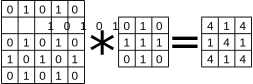
\includegraphics[scale=0.2]{img/konv-pelda.pdf}
		\captionsetup{justification=centering}
		\caption{Kétdimenziós konvolúció \textit{valid paddinggal}}
		\label{fig:conv-pelda-valid}
		
	\end{minipage}\hfill
	\begin{minipage}[c]{0.45\linewidth}
		\centering
		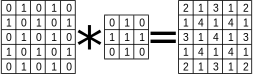
\includegraphics[scale=0.2]{img/konv-pelda-same-padding.pdf}
		\captionsetup{justification=centering}
		\caption{Kétdimenziós konvolúció \textit{same paddinggal}}
		\label{fig:conv-pelda-same}
		
	\end{minipage}
	
\end{figure}

%\begin{figure} [h!]
%	\centering
%	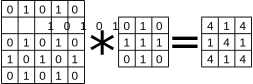
\includegraphics[scale=0.3]{img/konv-pelda.pdf}
%	\caption{Kétdimenziós konvolúció valid paddinggal}
%	\label{fig:conv-pelda}
%\end{figure}


%\paragraph{Dekonvolúciós reteg}
\subsubsubsection{Dekonvolúciós réteg}


A konvolúciós réteg inverze.
Autoencoder modellnél használjuk, mikor vissza szeretnénk állítani
a tömörített képet. Matematikailag ugyanaz mint a konvolúció,
a különbség csak az eredmény dimenziójában van.


\paragraph{Alul-mintavételező réteg} (\textit{Pooling, subsampling})


%Mély hálóknál az a célunk, hogy a dimenzió folyamatosan csökkenjen. Erre jó módszer, hogy a képet feleakkorára* csökkentjük, azaz négyesével összevonjuk a pixeleket, és valamilyen függvény segítségével kiszámoljuk belőlük az új értékeket.
%(\textit{* Lehet n-ed részére is csökkenteni a képet, nem csak a felére})

Mély hálóknál az a célunk, hogy a dimenzió folyamatosan csökkenjen. Erre jó módszer, hogy a képet feleakkorára\footnote{Gyakorlatban általában felezzük a képet, de használható bármilyen más, egész számú hányados is.} csökkentjük, azaz négyesével összevonjuk a pixeleket, és valamilyen függvény segítségével kiszámoljuk belőlük az új értékeket.



Ha jellemzővektorokkal dolgozunk, akkor legtipikusabb a \textit{Max pooling} réteg, ami a négy pixel maximumát veszi (\ref{fig:maxpooling-pelda}. ábra), de használatos még az \textit{Average pooling} is, amely az értékeket átlagolja. Ennek akkor van jelentősége, ha színértékekből álló képet szeretnénk alul mintavételezni.

% TODO ez a két ábra elrendezése egyszer már rossz volt az oldaltörés miatt! lecsekkolni hogy nem romlott e el

\begin{figure} [h!]
	\centering
	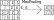
\includegraphics[scale=1.2]{img/max-pooling-pelda.pdf}
	\caption{Max pooling}
	\label{fig:maxpooling-pelda}
\end{figure}


\paragraph{Felül-mintavételező réteg} (\textit{Upsampling, Unpooling})


Az alul-mintavételezés ellentéte. Célja, hogy megtöbbszörözzük a réteg
méretét.



\begin{figure} [h!]
	\centering
	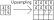
\includegraphics[scale=1.2]{img/upsamping-pelda.pdf}
	\caption{Felül-mintavételezés}
	\label{fig:upsampling-pelda}
\end{figure}




\subsubsection{Költségfüggvények}

Amikor a \ref{sec:kanonikus.feladat}. fejezetben definiáltuk a kanonikus tanulási feladatot, említettük, hogy az $ l(\underline{\hat{y}}, \underline{y}) $ függvényt költségfüggvénynek nevezzük. Nézzük most, hogy a dolgozatban milyeneket használunk.

%Általános alakban ha $ y $ az elvárt eredmény, és $ \hat{y} $ a háló
%outputja, akkor a hibafüggvény a következő:
%
%$ J(\underline{w}) = \dfrac{1}{n} \sumn{i} f(\underline{y}, \hat{\underline{y}}) $


\paragraph{Átlagos négyzetes hiba} (\textit{Mean square error, MSE})


\[  l(\underline{\hat{y}}, \underline{y}) = \norm{\underline{\hat{y}} - \underline{y}}_2^2  \]

\noindent
Akkor célszerű használni, ha tudjuk, hogy az eredmény nem lesz tökéletes, de szeretnénk mérni hibát. Az autoencodernél ezt használjuk.


\paragraph{Keresztentrópia} (\textit{Cross-entropy})

Legyen $ \underline{y} = (0, 0, \dots 1 \dots 0, 0)^T, $ 
ahol az 1 helye a hozzá tartozó osztály indexe.

Bináris esetben $ \underline{y}=(0, 1) $ ha a minta az első, és
$ \underline{y}=(1, 0) $ ha a második csoportba tartozik.

\[  l(\underline{y}, \underline{\hat{y}}) = - \underline{y}^T \cdot log(\underline{\hat{y}})  \]

\noindent
Osztályozásnál ezt használjuk.


\subsubsection{Kapcsolódó fogalmak}


\paragraph{Túltanulás} (\textit{overfitting})

%Egy modell akkor jó, ha a tanító példák mellett akkor is jól működik,
%ha olyan inputot kap, amilyet eddig még "nem látott". 
%
%Egy modell akkor jó, ha a tanító példák mellett új, még "nem látott"
%inputra is jól működik. Túltanulásnak nevezzük
%azt az állapotot, mikor az új adaton jelentősen romlik a teljesítmény.
%Ennek több oka is lehet. Például, ha az egyik osztályból nem kapott 
%(elég) mintaadatot a modell tanuláskor, vagy ha kapott is, a minták túlságosan 
%hasonlítottak egymásra, miközben a valóságban változatosabbak.
%Ennek kiküszöbölésére tekintsünk néhány módszert!


Egy modell akkor jó, ha a tanító példák mellett új, még "nem látott"
inputra is jól működik. Túltanulásnak nevezzük
azt az állapotot, mikor az új adaton jelentősen romlik a teljesítmény.
Ennek több oka is lehet. 

A legáltalánosabb, hogy a modellnek túl sok paramétere volt, és a tanító példákat tökéletesen megtanulta ahelyett, hogy összefüggéseket talált volna.

Túltanulást tapasztalhatunk akkor is, ha az egyik osztály sokkal több elemű volt mint a többi, ezáltal tanuláskor elnyomta a kisebbeket.

Ennek kiküszöbölésére tekintsünk néhány módszert!

%\paragraph{Hiperparaméterek}

\subsubsubsection{Hiperparaméterek}

Gépi tanulásnál megkülönböztetjük a modell belső változóit, amit 
a tanítás során az algoritmus maga számol, és a modell minden más tulajdonságát, amit a tervező ad meg. Utóbbiakat hívjuk \textit{hiperparamétereknek}. Ezek kiválasztása történhet próbágatással, vagy egy olyan algoritmussal, amely minimalizálni próbálja a validációs hibát \cite{bergstra2013hyperopt}.  
Hiperparaméter például egy kernel mérete, a tanulási együttható, vagy a rétegek szerkezete.



\subsubsubsection{Adat szeparálás}
%\paragraph{Adat szeparálás}

Bevett szokás, hogy ketté osztjuk az adathalmazt, az egyik részén tanítjuk a modellt (\textit{tanító halmaz, training set}), a másikkal ellenőrizzük, hogy mennyire teljesít jól a predikció (\textit{validációs halmaz, validation set}).

Ha csak ez a két halmazunk lenne, akkor előfordulhatna, hogy a hiperparaméterekkel addig-addig kísérletezünk amíg egyszer csak elfogadható validációs hibát kapunk. 
Lehetséges azonban, hogy ez az éppen kiválasztott adat sajátossága, azaz véletlen, ezért bevezetünk egy harmadik halmazt, a \textit{teszt halmazt}. Ennek célja, hogy ellenőrizni tudjuk a modell helyességét a hiperparaméterek véglegesítése után \cite{earlystopping}.


%, melynek célja, hogy
%mikor úgy ítéljük meg, hogy a validációs halmazzal elértük a kívánt eredményt,
%ellenőrizni tudjuk, hogy valóban jól teljesítünk-e.



Ideális esetben a validációs és a teszt hiba közel megegyező.


\paragraph{Kiejtés} (\textit{dropout})


A kiejtés célja, hogy a tanuló adatot szándékosan elrontsuk valamennyire, ezáltal növeljük az általánosítást és elkerüljük a túltanulást \cite{earlystopping}. Tartozik hozzá egy valószínűségi érték, amekkora eséllyel egy adatértéket kinullázunk mielőtt továbbadjuk a következő rétegnek.


%\paragraph{Kiegyensúlyozás}
\subsubsubsection{Kiegyensúlyozás}

Az eredményt torzíthatja, ha a tanító adatok között
nagy a relatív elemszámkülönbség: ezt nevezzük kiegyensúlyozatlanságnak.
Ennek kiküszöbölésére az egyik módszer, hogy minden halmazból 
megpróbálunk közel egyenlő eséllyel válogatni tanításnál. A másik megoldás, hogy az 
osztályoknak súlyokat adunk,
ami alapján paraméter állításnál jobban, vagy kevésbé fogja
az adott algoritmus figyelembe venni az adott példát. Az utóbbit több programcsomag is támogatja.

\paragraph{Adatgenerálás} (\textit{data augmentation})

Amennyiben nem áll rendelkezésünkre elég adat, és ez képeknél 
különösen gyakori probléma, úgy tudjuk növelni a tanító halmaz
elemszámát, hogy valós időben új adatokat generálunk a már
meglévők alapján \cite{krizhevsky2012imagenet}. Például egy képet affin transzformálunk,
vagy valamilyen hisztogram transzformációt alkalmazunk.


\subsubsection{A teljesítmény mérése}

Egy neuronháló tanítása általában hosszú folyamat. Ennek során valamilyen módszerrel meg kell
tudnunk állapítani, ha már elértük a kívánt eredményt és megállhatunk. Továbbá figyelnünk kell, 
hogy az optimalizálás abbahagyta-e a konvergálást, azaz elért egy 
lokális minimumot.
Ezen kívül mérni szeretnénk, hogy mennyire teljesítünk jól. 
Ezekre többféle metrika is létezik, ezek közül tekintünk néhányat.
Ezekhez vezessük be a következő bináris osztályozáshoz kapcsolódó fogalmakat:


Valódi-pozitív (\textit{true positive, tp}), 
Valódi-negatív (\textit{true negative, tn}): \\
Amikor egy példát megfelelően osztályozunk.

Fals pozitív / Elsőfajú hiba (\textit{fp}) 
és Fals negatív / Másodfajú hiba(\textit{fn}): \\
A mi kontextusunkban elsőfajú a hiba, ha egy hamisítványt eredetinek
osztályozunk, a másodfajú ennek fordítottja.

Azért fontos ezek kettéválasztása, mert ez a két hiba egymás rovására 
javítható. Egy adott feladatnál preferálhatjuk, hogy melyik az elfogadhatóbb.
Egészségügyben például kisebb kárt okozhat a fals pozitív, mint egy fals negatív;
mi viszont szívesebben engedünk át egy hamisítványt, mint mondjuk  azt egy eredetire, hogy hamis,
különben megrendülne a bankjegybe vetett bizalom.

% vagy emékezzünk a meghurcolt emberre, akinek a bkv bérletéről azt hitték hamis, pedig nem is

\subsubsubsection{Hisztogram}

Egy eloszlás megjelenítésére a legjobb módszer egy hisztogram készítése, amely véges számú, általában egyenközű intervallumra osztja az ábrázolandó halmazt, majd egy-egy intervallumhoz hozzárendeli, hogy hány minta esett bele. Közös hisztogramon tudunk ábrázolni több eloszlást is, ez kiváló arra, ha szemmel szeretnénk eldönteni, hogy szeparálható-e két adathalmaz. Erre láthatunk példát a \ref{fig:hist.pelda}. ábrán.

%Eloszlások vizualizációjára az egyik legjobb módszer


%\paragraph{ROC-görbe}
\subsubsubsection{ROC-görbe}


Az előző két hiba arányát a Vevő működési karakterisztika \cite{rocanalysis} (\textit{Receiver operating characteristic}) görbével szoktuk jellemezni. A két tengelyen az egyes hibák rátája található, és azt mutatja meg, hogy egy adott nagyságú elsőfajú hiba-rátához mekkora másodfajú tartozik. ROC-görbére a \ref{fig:roc.pelda}. ábrán láthatunk példát.

% TODO kicsit elcsúszott

\begin{figure}[h!]
	
	
	\begin{minipage}[c]{0.5\linewidth}
		\centering
		\includesvg[scale=0.5]{img/rocexample.svg}
		\caption{Egy ROC-görbe}
		\label{fig:roc.pelda}
		
	\end{minipage}\hfill
	\begin{minipage}[c]{0.5\linewidth}
		\centering
		\includesvg[scale=0.5]{img/histogram-ujratanitott-log-skala-test.svg}
		\caption{2 osztály hisztogramja}
		\label{fig:hist.pelda}
		
	\end{minipage}
	
\end{figure}



\paragraph{Pontosság} (\textit{accuracy}) \\
Azt méri, hogy az osztályozásnál a minták hányad részben
kerültek jó osztályba.
Ha $ (y_i, \hat{y_i}) $ az elvárt értékek és a hozzájuk tartozó 
predikciók, akkor

\[  acc = \dfrac{\sumn{i} \chi\{y_i = \hat{y_i}\}}{n}  \]

\noindent
Bár ez szemléletes, nem tükrözi igazán jól a hatékonyságot.


\paragraph{F1 score} \mbox{} 

\[  F_1 = \dfrac{2tp}{2tp + fn + fp}  \]

\noindent
Hasonló a pontossághoz, de jobb mérőszám, ha az osztályok kiegyenlítetlenek.



\paragraph{ROC görbe alatti terület} (\textit{ROC-AUC score})

Azt mutatja meg, hogy mennyire jól szeparálható a két adathalmaz. 
Ha az értéke 1, akkor tökéletesen elkülönül a két eloszlás, 
minél kisebb, annál rosszabb. Ha $ \frac{1}{2} $-nél kisebb számot kapunk,
akkor gyanakodhatunk, hogy felcseréltük a két osztályt.

\paragraph{Validációs hiba} (\textit{validation loss})

A korábban részletezett költségfüggvények eredménye. Ezt használjuk
tanítás közben annak mérésére, hogy a modell konvergál-e még,
és ha igen milyen sebességgel. Nem igazán szemléletes, végső kiértékelésnél
nem használjuk. Jó tulajdonsága, hogy nem csak azt méri, hogy jól
osztályozunk-e, hanem azt is hogy mennyire volt egyértelmű a döntés,
valamint félreosztályozásnál figyelembe veszi, hogy mekkorát hibáztunk.



\subsubsection{A tanítás menete}

Neuronháló tanításakor példákat mutatunk a modellnek, majd a kimenet
hibája alapján korrigálunk a súlyokon. Ezt a korrigálást viszont nem
minden minta után végezzük el, hanem kötegeket (\textit{mini batch}) 
készítünk, és ezek átlagos hibájával számolunk, ezáltal 
növelve a hatékonyságot és az általánosítást. Ügyelni kell azonban, hogy
akkora kötegméretet válasszunk, hogy beleférjünk a memóriába, ugyanis 
képeknél ez könnyen probléma lehet.


Bevált technika, hogy készítünk egy véletlen permutációt a tanító adatból,
és ebben a sorrendben adjuk be a példákat. Azt a ciklust, ami alatt 
az egész halmaz egyszer feldolgozásra kerül, \textit{eposz}nak hívjuk.
Eposzonként új permutációt használunk, ezekkel biztosítjuk, hogy minden
példa azonos valószínűséggel szerepeljen.

%\paragraph{Megállás}
\subsubsubsection{Megállás}

A megállási feltétel lehet explicit, például ha a validációs hiba egy előre
megadott érték alá csökken. Értelemszerűen megállunk, ha a tanulási hiba már nem csökken tovább.
Azonban könnyen előfordulhat, hogy az ugyan még egyre kisebb, a validációs hiba
viszont el kezd nőni! Ilyenkor biztosak lehetünk benne, hogy a modell elkezdett
túltanulni, ilyenkor megállunk (\textit{early-stopping}) \cite{earlystopping}.


%\paragraph{Regularizáció}
\subsubsubsection{Regularizáció}

%Ez a módszer arra való, hogy szabályozza a súlyok maximális méretét. Általában beleépítünk a 
%költségfüggvénybe  egy tagot, ami ezért felel. Például, ahogy az SVM-nél láthattuk:

Ez a módszer arra való, hogy szabályozza a súlyok maximális méretét, és mérsékelje a túltanulást \cite{regularizacio}. A \ref{sec:kanonikus.feladat} fejezetbeli általános feladatban a $ R(\theta) $ függvény volt a regularizáció. Például az SVM feladatnál:

%Például, ahogy az SVM-nél láthattuk:
%\underline{x}_1, \dots, \underline{x}_n, \underline{y}_1, \dots, \underline{y}_n

\[  L(\underline{w},b, \underline{x}_1, \dots, \underline{x}_n, y_1, \dots, y_n)  = \frac{1}{n} \sum\limits_{i=1}^{n} 
max(0, 1 - y_i(\underline{w}^T \underline{x}_i - b) + \lambda \norm{\underline{w}}  \]

\noindent
$  \lambda \norm{\underline{w}} $ a regularizációs tag, $ \lambda $ pedig egy hiperparaméter.





\newpage
\section{Megvalósítás}

A gépi tanulást két helyen vizsgáljuk a témakörben.
Először egy már meglévő applikáció mért eredményeit használjuk fel,
javítva a döntési folyamatot. Ehhez Támasztóvektor Gépet(SVM) használunk.
Másodszor konvolúciós hálók segítségével próbáljuk ugyanezt a döntést 
a nyers adatból, a képből meghozni. 

\subsection{Eszközök}

A megvalósítás nyelvének python-t választottunk.
A gépi tanuláshoz a \texttt{Keras}\footnote{\url{https://keras.io/}} \cite{chollet2015keras} és \texttt{Sklearn}\footnote{\url{http://scikit-learn.org/stable/modules/generated/sklearn.svm.SVC.html}} \cite{pedregosa2011scikit} könyvtárakat 
használtuk. Ezek a \texttt{Tensorflow}\footnote{\url{https://www.tensorflow.org/}} \cite{abadi2016tensorflow} csomag segítségével képesek a
GPU-n futni, ezáltal gyorsítva a tanítás folyamatát. Ez különösképpen a 
képfeldolgozásnál volt kritikus, mert egy közepes CPU és egy erős GPU között
százszoros sebességnövekedést mértünk.

Ahhoz, hogy a \texttt{Kerast} GPU-n tudjuk futtatni, szükségünk van az \texttt{Nvidia}
\texttt{Cuda}\footnote{\url{https://developer.nvidia.com/cuda-downloads}} csomagjára, amely a videókártya általános célú programozását 
segíti, valamint a \texttt{cuDNN}\footnote{\url{https://developer.nvidia.com/cudnn}} könyvtárra, amely mély neuronhálók tanításához 
szükséges komponensek hatékony implementációját tartalmazza. Fontos, hogy egyeztessük
össze a \texttt{Tensorflow} követelményeit az általunk letöltött \texttt{Nvidia} csomagokkal,
ugyanis azok nem visszafelé kompatibilisek.

Az említett csomagok az előző fejezetben leírt módszereket használva egy
keretrendszert biztosítanak, amellyel könnyen tudunk prototípusokat készíteni,
és azokat azonnal kipróbálni. Ezen kívül jól illeszkednek a python többi könyvtárához,
például a \texttt{numpy}\footnote{\url{http://www.numpy.org}} (általános aritmetikai könyvtár) és \texttt{opencv}\footnote{\url{https://opencv.org/}}
(computer vision, képfeldolgozás) csomagokhoz.


A továbbfejlesztendő program, a Jura Trade Kft. BPAS alkalmazása volt. Kezdetben ezzel legeneráltuk
a jellemzőinket az összes bemenetre, majd az eredményeket a \texttt{Bpas-Verdict.csv} és
a \texttt{Bpas-Merged.csv} fájlokba mentettük. Erről részletesen a \ref{sec:adatok}.
fejezetben írunk. Erre a programra a továbbiakban nem támaszkodtunk.



\subsection{Döntéshozás SVM-mel}

A kiinduló ötletünk az volt, hogy alkalmazzunk gépi tanulást egy már meglévő projektben,
és nézzük meg, hogy ezzel tudunk-e javítani rajta. Ez a meglévő projekt, bár több 
alkalmazás készült egy-egy ipari megoldáshoz, lényegében egy képet elemez 
különböző szempontok szerint, ez alapján fix darab számszerű jellemzőt készít, 
majd ezek alapján döntést hoz. Ez az algoritmus minden alprojekthez egyesével
volt kézzel megírva a szakértői tapasztalatok alapján. 

Ezt a mechanizmust szerettük volna automatizálni. Abban reménykedünk, hogy egy 
mesterséges intelligencia esetleg olyan összefüggéseket is felismerhet a jellemzők
között, ami felett az ember esetleg elsiklik, valamint ha csak küszöbválasztásra
gondolunk, egy elemi döntésnél biztonságosabbnak tűnik azt automatikusan, statisztikai
alapokon beállítani, mint kézzel kikísérletezni, hogy az adott példákra mikor működik jól.
További előny, hogy ha akár ugyanabba a projektbe új minta érkezik, gondoljunk például újféle 
hamisítványra, akkor az újratanítást automatikusan el lehet végezni az új adathalmazon,
nem kell hozzá új algoritmust kitalálni. Amennyiben folyamatosan nő az adathalmazunk, 
bizonyos időközönként akár automatikusan is tudunk új szoftververziót készíteni,
ami jobban illeszkedik az új mintákhoz, és biztonságosabban ítél.


A jellemző adatokra fekete dobozként tekintettünk, semmilyen formában nem használtuk fel
a jelentésüket, tehát hagytuk hogy a gép magától találjon összefüggéseket.


Építhettünk volna egy neurális hálót is, de sokkal egyszerűbb, mégis hatékony
megoldásnak bizonyult az SVM, amely kiváló ilyen bináris adat-klaszterezésekre.
További előnye, hogy viszonylag kevés mintán is jól és gyorsan tud tanulni.
Mindezek mellett kevesebb a hiperparamétere.


\subsubsection{Adatok}
\label{sec:adatok}

Az adatainkat egy \texttt{csv} fájlból olvassuk ki, amit az előzőekben említett program 
generált. Egy-egy sor tartalmazza az adott fájl elérési útját, a \textit{ground truth}-t,
a Jurás program predikcióját, néhány metaadatot, és végül a számunkra érdekes jellemzőket.
Körülbelül 1000 mintánk állt rendelkezésre.

\noindent
A következő két adatfájlt használtuk:

\begin{enumerate}
\item
	\texttt{bpas-verdict.csv}: Minden egyes kép adatai egyszer szerepelnek
\item
	\texttt{bpas-merged.csv}: Az egymáshoz tartozó képek közül csak a jobbik szerepel benne
\end{enumerate}

Egy sor esetlegesen tartalmazhat hibaüzenetet, ha a képet nem sikerült előzetesen elemezni, például 
ha annyira homályos, hogy célzóköröket nem sikerült megtalálni. Az ilyen sorokat figyelmen kívül hagyjuk.

Tekintve, hogy a tanítás időtartama alatt nem változnak az adatok, a kézzel adjuk
meg a jellemzők oszlopindexeit. A kódban ez:
\begin{lstlisting}  
	valueableParamIndices = [18, 20, 22, 24, 26, 27, 29, 30, 32, 33, 35, 36, 38, 39, 41, 42]
\end{lstlisting}

Ezeket a rekordokat kigyűjtöttük egy $ x $ tömbbe, az elvárt eredményeket egy $ y $-ba:
ezek lesznek a modellünk paraméterei.



\subsubsection{A modell}

Az SVN-ünket az \texttt{Sklearn} csomag \texttt{SVC} osztálya segítségével építjük fel. A következőekben ennek paramétereit tárgyaljuk.

% kell ide a kód? vagy fölösleges
%
%\begin{lstlisting}  
%
%
%	clf = SVC(
%			C=1., 
%			cache_size=200, 
%			class_weight=class_weight, 
%			coef0=0.0,
%			decision_function_shape=None, 
%			degree=2, 
%			gamma='auto', 
%			kernel='rbf',
%			max_iter=-1,
%			probability=True, 
%			random_state=None, 
%			shrinking=True,
%			tol=0.001, 
%			verbose=False)
%
%\end{lstlisting}



%\subsubsection{Hiperparaméterek}

\subsubsection{Kernelek}

%http://scikit-learn.org/stable/modules/svm.html#svm-kernels

Mint azt a \ref{sec:kernelek}. fejezetben írtuk, a kernelek feladata, hogy megnöveljék a probléma
dimenzióját annak érdekében, hogy az így lineárisan szeparálhatóvá váljon, mindezt 
úgy, hogy meglévő jellemzőpárokból újakat generálnak előre megadott képletek,
bázisok segítségével. Nézzük \texttt{sklearn}-ben milyen lehetőségeink vannak a 
kernel függvények megadására.

\begin{itemize}
\item
	\textbf{Lineáris:} \\
	\texttt{SVC.kernel='linear'}
\item
	\textbf{Polinomiális:} \\
	\texttt{SVC.kernel='poly'}	\\
	\texttt{SVC.degree} $ \rightarrow d $ \\
	\texttt{SVC.coeff0} $ \rightarrow r $
\item 
	\textbf{Radiális Bázis Függvények:} \\
	\texttt{SVC.kernel='rbf'}	\\
	\texttt{SVC.gamma} $ \rightarrow \gamma $
\item 
	\textbf{Szigmoid:} \\
	\texttt{SVC.kernel='sigmoid'}	\\
	\texttt{SVC.coeff0} $ \rightarrow r $
\end{itemize}
%
%\paragraph{Lineáris} (\texttt{linear})
%% TODO aláhúzásokra figyelni
%%TODO képletek legyenek a háttérben
%
%\[  k(x, x') = \underline{x}^T \cdot \underline{x}'  \]
%
%
%\paragraph{Polinomiális} (\texttt{poly})
%
%\[  k(x, x') = (\gamma \cdot (\underline{x}^T \cdot \underline{x}') + r)^d  \]
%
%\texttt{SVC.degree} $ \rightarrow d $
%
%\texttt{SVC.coeff0} $ \rightarrow r $
%
%\paragraph{Radiális Bázis Függvények} (\texttt{rbf})
%
%
%\[  k(x, x') = exp( - \gamma \cdot \norm{\underline{x} - \underline{x}'}^2)  \]
%
%\texttt{SVC.gamma} $ \rightarrow \gamma $
%
%
%
%
%\paragraph{Szigmoid} (\texttt{sigmoid})
%
%\[  k(x, x') = tanh(\gamma \cdot (\underline{x}^T \cdot \underline{x}') + r)  \]
%
%\texttt{SVC.coeff0} $ \rightarrow r $


\noindent
Mi a dolgozatban végül \texttt{RBF} kernelt használtunk.

\subsubsection{Egyéb paraméterek}

\subsubsubsection{SVC.class\_weight}

Amennyiben az adatunk kiegyensúlyozatlan (márpedig nekünk az), ezzel adhatjuk meg
 egy-egy osztály súlyát, amely általános esetben fordítottan arányos az elemszámmal.

Ehhez használtuk a csomag \texttt{compute\_class\_weight} függvényét, ami éppen ezt csinálja.
Paramétere  kívánt osztályok, és \textit{ground truth}-ok.


\subsubsubsection{SVC.tol}

Hibatolerancia. Ha ezt elértük, akkor abbahagyhatja a modell a tanulást.



%The C parameter trades off misclassification of training examples against simplicity of the decision
%surface. A low C makes the decision surface smooth, while a high C aims at classifying all training
%examples correctly by giving the model freedom to select more samples as support vectors

\subsubsubsection{SVC.C\footnote{\url{http://scikit-learn.org/stable/auto_examples/svm/plot_rbf_parameters.html}}}  

%Regularizációt\footnote{\url{http://scikit-learn.org/stable/auto_examples/svm/plot_svm_scale_c.html}} szabályozó paraméter. Ha visszatekintünk az SVM költségvényének alakjára:
%% TODO lehet hogy elég egy visszautalás, a megvalósításban már ne legyen képlet
%
%%$ J(\underline{w},b)  = \frac{1}{n} \sum\limits_{i=1}^{n} 
%%f(x_i, y_i) + \lambda \norm{\underline{w}} $
%
%\noindent
%Ekkor az \texttt{sklearn} $ C $ paramétere megegyeztethető $ \frac{1}{\lambda} $-val.
%Ha $ C $ kicsi, akkor simább a döntési felület és egyszerűbb modell, ha nagyobb, akkor 
%jobban próbál specializálni. Az első eset a túl nagy általánosság, a második a túltanulás
%miatt lehet problémás.

Regularizációt\footnote{\url{http://scikit-learn.org/stable/auto_examples/svm/plot_svm_scale_c.html}} szabályozó paraméter. Ha visszatekintünk az SVM költségfüggvényének alakjára a \ref{sec:svm}. fejezetben, akkor az \texttt{sklearn} $ C $ paramétere megegyeztethető $ \frac{1}{\lambda} $-val.
Ha $ C $ kicsi, akkor simább a döntési felület és egyszerűbb modell, ha nagyobb, akkor 
jobban próbál specializálni. Az első eset a túl nagy általánosság, a második a túltanulás
miatt lehet problémás.



% jobb cím?
\subsubsection{Tulajdonságok}

\noindent
A tanítás $ \mathcal{O}(n^2) $ futási idejű, ezért nem jól skálázható. Bár a mi 
esetünkben kiválóan működött, a csomag dokumentációjában azt olvashatjuk, hogy néhány tízezernél
több mintára már nem alkalmazható hatékonyan.


Magát a tanítást a modellünk \texttt{fit(x, y)} függvényével tudjuk elvégezni, ezután 
a \texttt{predict} metódussal tudunk egy-egy mintát osztályozni.



\subsubsection{Hiperparaméter optimalizálás}
\label{sec:svm.hiperparameter.optimalizalas}

Ahogy korábban láthattuk, még az egyes kernelekhez is többféle hiperparaméter választható. Ezek kiválasztása
feladatfüggő, és nem triviális. Egy hiperparaméter jóságát a validációs hibával mérjük. Ennek 
bevett módja a \textit{validation loss} mérése, aminek egy változata ugyan előállítható lett volna 
az osztály valószínűségekből, mégis kézenfekvőnek tűnt egy másik mértéket bevezetni: az átlagos hibarátát.

Az alapvető probléma az volt, hogy ha 1000 elemű a teljes mintahalmaz , akkor a validációs 
halmaz ennél mindenképp kisebb. 

Az alapvető probléma az volt, nem volt elég nagy a teljes mintahalmaz, és ezáltal a validációs halmaz.
A hibás klasszifikációk rátája kb. $ 0.01 $ volt az alapértelmezett paraméterek mellett, ami azt
jelenti, hogy kb. 10 darab hiba volt egy validációs halmazban. Ennek a számnak a szórását mérve véletlenszerű
tanító-tesztelő halmaz szeparációk mellett azt találtuk, hogy nem megbízható statisztika a 
hiba ilyen módon történő mérése.

Ezért valahányszor egy hiperparaméter kombinációt próbáltunk, újra és újra lefuttattuk a
tanítást különböző felosztásokra, és ennek az átlagával számoltunk. Így kielégítően nagy 
konfidencia mellett mondhatjuk, hogy ha egy hiperparaméter halmaz ilyen módon is jó eredményt
produkál, akkor nem fogja jelentősen befolyásolni a tanító halmaz megválasztása a validációs 
eredmény eloszlását.

A legjobb hiperparaméterek megtalálásához a \texttt{hyperopt}\footnote{\url{https://github.com/hyperopt/hyperopt}} csomagot vettük
igénybe. Használatához meg kell adjuk, hogy milyen változókat milyen valószínűségi eloszlás szerint
mintavételezzen. Ezután a \texttt{fmin} függvényt meghívva a keretrendszer elkezdi véletlenszerűen
kipróbálni a modellünket az egyes hiperparaméterekkel, majd visszatér a legjobbal. 

Mi a \texttt{SVC.C} és a \texttt{SVC.gamma} paramétereket kerestük a [-0.001, 1000] intervallumban,  logaritmikusan egyenletes eloszlást használtunk, és 100 helyen értékeltük ki.
%
%Az általunk használt konfiguráció a következő volt:
%% szinezni
%
%\begin{lstlisting}
%
%
%	from hyperopt import fmin, tpe, hp, STATUS_OK, Trials
%	
%	low = np.log(1e-3)
%	high = np.log(1e+3)
%	
%	fspace = {	
%		'C': hp.loguniform('C', low, high),
%		'gamma': hp.loguniform('gamma', low, high)
%	}
%	
%	def f(params):
%		C = params['C']
%		gamma = params['gamma']
%		fpr, fnr = batch_fit_and_test(x, y, file_names, N=200, gamma=gamma, C=C)
%		val = fpr + fnr
%		return {'loss': val, 'status': STATUS_OK}
%	
%	trials = Trials()
%	best = fmin(fn=f, space=fspace, algo=tpe.suggest, max_evals=100, trials=trials)
%	
%	# futtatas vegen:
%	# best: {'C': 6.250906239883302, 'gamma': 0.03357455814119452}
%\end{lstlisting}


A legjobb eredményt a $ C=6.25 $ és $ \gamma = 3.3 \cdot 10^{-2} $ paraméterekkel érte el $ 100 $
mintavételezésből. Ez természetesen hosszabb futtatással javítható. Látható viszont, hogy a csomag
beépített paraméterei ($ C=1 , \gamma =\dfrac{1}{len(samples)} $) ehhez nagyságrendileg elég közel vannak,
és alkalmasak a tanításra.


\subsubsection{Dupla képes eljárás}
\label{sec:dupla.kepes.eljaras}

A dolgozat alapjául szolgáló alkalmazás úgy működött, hogy a nagyobb biztonságért két képet készített
egymás után, hogy ha az egyik valami miatt rossz minőségű lett, akkor ki tudjuk választani a jobbat, 
és azt elemezni. Ezt mi is megpróbáltuk kihasználni. A \texttt{csv} fájlban az egymás után készült képek adatait
összefűztük. Két ilyen fájlt onnan ismerünk meg, hogy csak egy \texttt{\_0.png} és \texttt{\_1.png}
posztfixben térnek el.

Ezek alapján három tanító módszert tudunk készíteni.:
\begin{enumerate}
	\item
	Minden egyes képhez rendelünk egy döntést.
	Adat: \texttt{bpas-verdict.csv}*
	\item 
	Minden, már eleve egybeolvasztott adatot úgy kezelünk, mintha az csak 
	egy kép lenne. Adat: \texttt{bpas-merged.csv}*
	
	\item 
	A képek jellemzőit a fentiek szerint az input fájlból egymás mögé 
	fűzünk, és az alapján dolgozunk.
	Adat: \texttt{bpas-verdict.csv}*
\end{enumerate}

\textit{*Lásd a \ref{sec:adatok} pontot.}
%
%négyzetes tanítási idő, nem működik 100k példára
%az svm kvázi determinisztikus
%
%* valahova beleirni hogy kevés mintán is tud üzemelni
%
% az svm többi paraméterét leírni
% ? és az az általánosba kell vagy ide? 
%
%
%
%voltak random adatok
%nincs szükség arra hogy tudjuk mit jelentenek a mért adatok
%általános
%minden projekt ilyen elveken mukodott, bármelyikre lehet alkalmazni
%verdict
%hasonlóan működött az eredeti algo cska kézzel volt minden megcsinálva


\newpage
\subsection{Képelemzés Konvolúciós Hálóval}
\label{sec:cnn}


\subsubsection{Adatok}


\begin{figure}[h]
	
	
	\begin{minipage}[c]{0.5\linewidth}
		\centering
		\includegraphics[width=\textwidth]{img/eredeti-pelda.png}
		\caption{Eredeti nyomat}
		\label{fig:eredeti.pelda}
		
	\end{minipage}\hfill
	\begin{minipage}[c]{0.5\linewidth}
		\centering
		\includegraphics[width=\textwidth]{img/copy-pelda.png}
		\caption{Színes fénymásolat}
		\label{fig:copy.pelda}
		
	\end{minipage}
	
\end{figure}

Ennél a megközelítésnél maguk a képek voltak a tanító adatok. Ezekre láthatunk példát a  \ref{fig:eredeti.pelda}. és a \ref{fig:copy.pelda}. ábrán.
Mivel a képek érkezhetnek különböző felbontású forrásokból, célszerű volt
egyformára méreteznünk őket. Ennél tovább mentünk, és a célzó körök koordinátáival,
és az \texttt{opencv} könyvtár inverz perspektivikus transzformációja segítségével 
normalizáltuk a képeket. Végeredménynek egységesen $ 1000 \times 1000 $ pixeles képeket
választottunk. Az \ref{fig:normalized-eredeti.pelda}. és a \ref{fig:normalized-copy.pelda}. 
ábrán láthatjuk a normalizálás eredményét.


\begin{figure}[h]{}
	
	\begin{minipage}[r]{0.5\linewidth}
		\centering
		\includegraphics[width=0.8\textwidth]{img/normalized-eredeti-pelda.png}
		\caption{Normalizált eredeti nyomat}
		\label{fig:normalized-eredeti.pelda}
		
	\end{minipage}\hfill
	\begin{minipage}[l]{0.5\linewidth}
		\centering
		\includegraphics[width=0.8\textwidth]{img/normalized-copy-pelda.png}
		\caption{Normalizált színes fénymásolat}
		\label{fig:normalized-copy.pelda}
		
	\end{minipage}
	
\end{figure}

A célzó koordináták már rendelkezésünkre álltak, de jó kutatási terület lehet ezek 
megtalálása egy erre készített neurális hálóval.


Összességében azt várjuk, hogy a háló az eredeti és a hamis képeken más-más 
jellemzőket talál és tanul meg a konvolúciós szűrők segítségével, és ezeket
a \textit{feature-öket} a sűrű háló már könnyen kategorizálni tudja.

Ahogy azt a mély hálóknál szokás, a rétegek fokozatosan csökkentik a probléma
dimenzióját (kezdetben a teljes kép), amíg el nem érjük a keresett választ, azaz 0 vagy 1 - 
egy dimenzió.

\subsubsection{A háló szerkezete}

Bár több konfigurációt kipróbáltunk, a szerkezet alapvetően mindig a következő:



\begin{enumerate} [itemsep=-1ex]
	\item Bemenet
	\item Konvolúciós + alul mintavételező rétegek
	\item Sűrű rétegek
	\item Osztályozó réteg
	\item Predikció
\end{enumerate}

%A végső szerkezet Keras segítségével megvalósítva:
\textbf{A végső modell}:
% konv lokális, dense nem
% tikz, vagy rajz
% TODO ellenőrizni a nyomtathatóságot
\begin{figure} [h!]
	\label{fig:predictor-halo-modell}
	\centering
	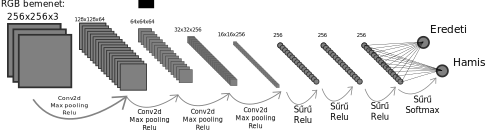
\includegraphics[scale=0.3]{img/predictor-network-modell.pdf}
	\caption{A háló modellje}
\end{figure}

%
%\lstset{language=Python}
%\begin{lstlisting}  
%	model = Sequential()
%	model.add(Conv2D(64, (5, 5), input_shape=input_shape))
%	model.add(Activation('relu'))
%	model.add(MaxPooling2D(pool_size=(2, 2)))
%	
%	model.add(Conv2D(64, (5, 5)))
%	model.add(Activation('relu'))
%	model.add(MaxPooling2D(pool_size=(2, 2)))
%	
%	
%	model.add(Conv2D(256, (5, 5)))
%	model.add(Activation('relu'))
%	model.add(MaxPooling2D(pool_size=(2, 2)))
%	
%	model.add(Conv2D(256, (5, 5)))
%	model.add(Activation('relu'))
%	model.add(MaxPooling2D(pool_size=(2, 2)))
%	
%	
%	model.add(Flatten())
%	model.add(Dense(256))
%	model.add(Activation('relu'))
%	
%	model.add(Dense(256))
%	model.add(Activation('relu'))
%	
%	model.add(Dense(256))
%	model.add(Activation('relu'))
%	
%	
%	model.add(Dropout(0.5))
%	model.add(Dense(2))
%	model.add(Activation('softmax'))
%	
%	
%	model.compile(
%		loss='sparse_categorical_crossentropy',
%		optimizer='adam',
%		metrics=['accuracy']
%	) 
%
%\end{lstlisting}


Az $ 5 \times 5 $-ös kerneleket \textit{Relu} nemlinearitással találtuk legcélszerűbbnek,
valamint $ 2 \times 2 $ \textit{max pooling}ot minden réteg után.
A konvolúciós és a sűrű rétegek között egy \textit{Flatten} réteg található,
ami a $ \mathbb{R}^{w \times h \times d} $ három dimenziós mátrix formából 
$ \mathbb{R}^{w \cdot h \cdot d} $ vektort képez. Ezután további sűrű rétegek
következnek \textit{Relu} nemlinearitással. Az utolsó az osztályozó
réteg, amelynek két eleme van, és a \textit{softmax} függvény segítségével kapjuk
a háló válaszát. Ez kategóriánként egy 0 és 1 közötti valós szám, ahol a kategóriák 
összege 1 (ld. softmax függvény definíció). Bár nincs közük a valószínűségszámításhoz, 
ezek a számok felfoghatók úgy, hogy mekkora eséllyel tartozik a minta az adott osztályba.
Amennyiben közelebb vagyunk nullához vagy egyhez, akkor magabiztosabb a becslés, 
$ \frac{1}{2} $ esetén bizonytalan.

Költségfüggvénynek \textit{keresztentrópiát} használunk. Ez végtelen nagy ha $ |y-y'|=1 $,
és 0, ha $ |y-y'|=0 $. Vegyük észre, hogy a \textit{softmax} miatt csak akkor lesz 0
a költség, ha az egyik osztály pontosan 1, a másik pedig pontosan 0.

A keresztentrópiának több változata létezik, de ezek csak az input formájában térnek
el. Lehet például általános $ n $ elemű, bináris két elemű, vagy bináris egyváltozós.
Mi az általános esetet használtuk, de a három közül bármelyik megfelelt volna.


\subsubsection{Tanítási paraméterek}

%\paragraph{Kötegméret}

\subsubsubsection{Kötegméret}

\nopagebreak

Megválasztásakor arra törekedtünk, hogy minél nagyobb legyen, ezzel gyorsítva a feldolgozást.
Ekkor matematikailag is magabiztosabb a konvergencia egy határig, 
valamint a GPU-RAM átviteli sávszélessége hiába nagy, de jelentős a konstans késleltetés, 
ami abból adódik, hogy a videókártya vezérlőszoftver nem azonnal hajtja végre az adatmozgatást,
hanem csak ha elég sok összegyűlt, vagy némi idő eltelt, ezzel javítva az teljesítményt teljes 
kihasználtság esetén. Egy eposz feldolgozása akár tízszer lassabb is lehet, ha a példákat
egyesével tápláljuk be.



\label{gpu.memory}
\textit{Megjegyzés}: Talán hiba, de mindenesetre létező jelenség a Tensorflow csomagban, ha GPU implementációt használunk a program betöltéskor megpróbálja a lehető legtöbb 
munkamemóriát lefoglalni magának, ami nem mindig sikerül, 
ezért előfordulhat hogy hibával elszáll a program. Erre jó megkerülő megoldásnak bizonyult, hogy
korlátoztuk a maximálisan lefoglalható memória mennyiségét. Erre szolgál a következő utasítás a kódban:
\begin{lstlisting}
	config.gpu_options.per_process_gpu_memory_fraction = 0.7
\end{lstlisting}


Felmerül a kérdés, hogy miért nem mindent a GPU-n tárolunk, ezzel megspórolva az adatmozgatást.
Sajnos körülbelül 1000 tanító képünk volt, $ 1600 \times 1600 $ felbontásban. 
Tömörítetlenül ez nem fért el a memóriában. Ezt később ugyan lecsökkentettük
$ 1000 \times 1000 $-re, így elméletben már elfért volna, de ez nem került implementálásra,
mert hosszú távon több kép esetén úgyis probléma lenne.



Találkozhatunk egy figyelmeztető üzenettel, ha elfogy a memória, ami bár nem 
okoz végzetes hibát, de ilyenkor lassabban fut a program. Ezért érdemes úgy megválasztani
a paramétereket, hogy ez ne következzen be.


Ezek miatt a kötegeket dinamikusan töltjük be a lemezről, és adjuk át feldolgozásra.
Egy köteg mérete jelenleg 16, de ez erősebb vagy gyengébb hardver függvényében 
növelhető vagy csökkenthető. A jelenlegi modellméret és képfelbontás mellett, ez 
körülbelül a határ a tesztgépen. Ez abból adódik, hogy a Keras felépíti memóriában 
a teljes futószalagot (\textit{pipeline}), ami csak az első rétegben
$ 3 \times 1000 \times 1000 \times 256 $ bájt memóriát foglalna.
Ezt kicsivel csökkentettük azzal, hogy a képeknek csak az egyik, jobb felső,
$ 256 \times 256 $ pixeles sarkát használtuk fel. A kísérletek szerint ez nem okozott
jelentős minőségromlást, de természetesen egy éles, ipari környezetben ez nem lenne
elhanyagolható.


%\paragraph{Képformátum}
\subsubsubsection{Képformátum}


Az \texttt{opencv} könyvtárat használjuk a képek betöltésére.
A bemeneti képeink fájlformátuma bármi olyan lehet, amit az \texttt{opencv} támogat.
Mi \texttt{PNG}-t használunk a veszteségmentes tömörítés miatt, de nem elképzelhetetlen
a \texttt{TIFF} sem.


A \texttt{cv2.imread()} függvény egy 8 bites egészeket
tartalmazó \texttt{numpy} tömbbel tér vissza. Mi ezzel szemben lebegőpontos számokkal számolunk,
ezért 0 és 1 közé transzformáljuk a bemenetet. Ez a modell szempontjából irreleváns lenne,
de ha az ember ilyen képeket szeretne hibakeresés céljából megjeleníteni, akkor a
könyvtári megjelenítő függvények konvencionálisan ilyen értékeket várnak.


A képek reprezentációja könyvtáraktól függően különbözhet továbbá az egyes dimenziók 
sorrendjében, ezért fontos hogy konzisztensek legyünk. Mi az \texttt{opencv}-hez
igazodtunk, ahol a tömb \textit{alakja (shape)} : 
$ \mathbb{R}^{height \times width \times channels } $. 
Tehát egy pixel három színe három, fizikailag egymás mellett lévő érték,
míg más reprezentációkban előfordul, hogy a csatornák vannak elől, azaz három különálló
szürkeárnyalatos képünk van.


%\paragraph{Adathalmaz}
\subsubsubsection{Adathalmaz}

Körülbelül 1000 kép állt rendelkezésünkre tanításkor, ezek 80\%-a volt
eredeti, a maradék 20\% hamisítvány. 


Emiatt szükséges volt a mintát kiegyensúlyozni, tehát gondoskodni arról,
hogy a tanításnál mindkét csoportból azonos valószínűséggel lásson mintát 
a modell. Az egyik, kevésbé elegáns módszer szerint a kisebb (negatív) 
halmazból addig szúrtunk be mintákat véletlenszerűen a tanító minták közé, 
amíg egyenlő nem lett a két halmaz elemszáma.
Ennél szofisztikáltabb megoldás, a \texttt{Keras} \texttt{class\_weights} paraméterét
használni, amellyel megadhatjuk, hogy egy-egy osztályt milyen mértékben vegyen 
figyelembe a tanításnál. Az \texttt{sklearn} csomag biztosít egy függvényt,
\texttt{sklearn.utils.compute\_class\_weight} néven, vagy kézzel könnyen kiszámolhatjuk 
magunknak:

\[  w_k' =  \dfrac{n}{ \sumn{i} \chi\{y_i = k\}}   \]

\[  w_k =  \dfrac{w_k'}{\sumn{i} w_i'}  \]


A képek különböző telefonokkal készültek, némely állványról, a többi pedig kézből.
Ez nagyban tudja befolyásolni a képminőséget.


Tanítás előtt képezünk egy tanító, egy validációs és egy teszt halmazt, ahol 
$ 70:15:15 $ az elemek számának aránya. Ezután, hacsak nem volt változás az adathalmazban,
ezeket használtuk a végsőkig.



%\paragraph{Adat augmentálás}

\subsubsubsection{Adat augmentálás}

Fent írtunk arról, hogy ha relatív kevés tanító adatunk van, hogyan is tudunk
ezekből újakat generálni. Képfeldolgozással foglalkozó témákban ez azt jelenti,
hogy valamilyen affin transzformációt hajtunk végre a képen, ezáltal növelve a 
generalizálást. Viszont mivel mi a kezdő lépésben normalizáljuk a képünket azzal,
hogy a négy célzópontot egy négyzetté transzformáljuk, elveszítjük ennek a módszernek
a jelentőségét.


Jó kutatási terület lehet, hogy ezt hogyan lehet feladatspecifikusan és valósághűen 
mégis véghez vinni, például a fényviszonyok változásának szimulálásával.

\subsubsubsection{Dropout} 

Továbbra is működik véletlenszerű kiejtés módszere,
azaz tanítás során két réteg között az áramló adat véletlenszerűen elveszik
egy előre megadott valószínűségi változó szerint. Mi $ p=0.5 $ egyenletes 
eloszlást használtunk. Ez a módszer jó mind konvolúciós, mind a sűrű rétegekre.



\subsubsubsection{Optimalizáló}

Ahogy az korábban írtuk, a tanítás problémáját tulajdonképpen visszavezettük egy numerikus optimalizációs feladatra. Erre több módszer létezik, de általában a Gradiens Módszeren alapulnak. Mi az Adaptív Momentum Becslés (\textit{Adaptive Moment Estimation, Adam~\cite{kingma2014adam} }) módszert használtuk. Erről bővebben a \ref{sec:adam}. fejezetben írtunk.
%
%\noindent
%Az algoritmus röviden:
%
%\[  m_w^{t+1} = \beta_1 \cdot m_w^{t} + (1-\beta_1) \triangledown_w J(w_t)  \]
%
%\[  v_w^{t+1} = \beta_2 \cdot v_w^{t} + (1-\beta_1) (\triangledown_w J(w_t))^2  \]
%
%\[  \hat{m}_w = \dfrac{m_w^{t+1}}{1 - \beta_1}  \]
%
%\[  \hat{v}_w = \dfrac{v_w^{t+1}}{1 - \beta_2}  \]
%
%$ w^{t+1} = w^{t} - \gamma \dfrac{\hat{m}_w}{\hat{v}_w + \epsilon}   $
%
%\noindent
%,ahol $ \beta_{1,2} $ a felejtési együtthatók, $ \gamma $ a tanulási együttható,
%$ w $ az optimalizálandó paraméter, és $ J $ a költségfüggvény.
%
%\noindent
%\texttt{Kerasban} az alapbeállítások: 
%$ \beta_1=0.9, \beta_2=0.999, \epsilon=1e-08, \gamma=0.001 $
%
%%Keras: lr=0.001, beta_1=0.9, beta_2=0.999, epsilon=1e-08, decay=0.0.


\subsubsection{Modell készítés}

A paraméterek függvényében ellenőrizzük, hogy elérhető-e előző munkamenet.
Ha igen, akkor megpróbáljuk betölteni. Az elmentett modell kétféle lehet:

\begin{samepage}
	\begin{itemize}
		\item 
		"Csak súlyok"; csak akkor van értelme, ha már végleges verziónk van.
		
		\item 	
		"Teljes modell"; ahol a súlyok mellett a háló szerkezete, és az optimalizáló állapota
		is elmentésre kerül.
	\end{itemize}
\end{samepage}





Ezután két részre bontottuk a feladatot, amelyek egymástól függetlenül futtathatók.
Az első a háló tanítása (akár meglévő finomítása), a második a modell használata 
és statisztikai értékelése.

\subsubsection{Első fázis}

Amikor elkészült a modell, akkor készen állunk a tanításra. Ha teljes modellt töltöttünk be,
akkor pont onnan folytatjuk, ahol abbahagytuk. "Csak súlyok" esetén jelentősen visszaesünk 
eleinte, modell nélkül pedig "nulláról"(véletlenszerűen inicializált állapotból) kezdünk.

Az effektív tanítás \texttt{keras.models.Sequential.fit\_generator()} metódus segítségével 
történik.

Ennek a paramétereiként meg kell adnunk a tanító és a validációs halmazokat \texttt{python} 
generátorok formájában. Ezek olyan \texttt{numpy} tömbökkel térnek vissza, amely megfelelnek 
egy-egy kötegnek, és egy-egy eleme egy kép. A \texttt{steps\_per\_epoch} paraméter segítségével azt adjuk
meg, hogy egy \textit{eposz} hány köteg. A \texttt{callbacks} paraméterrel függvényeket
adunk a modellnek, amelyek bizonyos események bekövetkeztével meghívódnak. Tipikusan a
\texttt{on\_epoch\_end} callbacket használtuk.

\noindent
A következőket definiáltuk:

\paragraph{Korai megállás} (\textit{Early stopping})

Nem a \texttt{Keras} beépített függvényét használtuk, hanem sajátot írtunk a
nagyobb szabadság miatt. A feladata, hogy ha a validációs hiba már nem csökken, akkor 
szakítsa meg a tanítást. Viszont azt tapasztaltuk, hogy előfordul, hogy néha
egy-egy eposz erejéig a hiba nő, ámde a következőben újra stabilan csökken.
Ezért csak akkor állunk meg ha a validációs hiba három egymást követő eposzban
nem csökkent.

\texttt{Kerasban} a validációs hibát a \texttt{on\_epoch\_end(self, epoch, logs=\{\})} 
callback függvényben a \texttt{logs.get(self.monitor)} utasítással kapjuk meg.

Megadhatunk explicit legtöbb eposz-számot is, és validációs hibahatárt, ami alá ha
elérünk akkor elvégezettnek tekintjük a feladatot, de ezt a gyakorlatban nem használtuk.
Addig tanítottuk, ameddig csak lehetett.

%\paragraph{Ellenőrzőpont}
\subsubsubsection{Ellenőrzőpont}

Mivel a tanítás hosszú folyamat, eközben akár össze is omolhat a rendszer, vagy
a modell elkezdhet egy idő után \textit{túltanulni}. Többek között ezek miatt fontos,
hogy rendszeres időközönként elmentsük a jelenlegi állapotot. Ehhez egy 
\textit{Checkpoint~Callbacket} implementáltunk, amely a jelenlegi verzióban minden ötödik
eposz után a lemezre menti a modellt, ellátva egy időbélyegzővel.



\subsubsection{Második fázis}
\label{sec:masodik.fazis}

A második fázisban egy már betanított modellt használunk. Ekkor már tudunk predikciókat 
végezni, és ezáltal hatékonyságot mérni. A bináris osztályozó tulajdonsága, hogy bár
a formátum különbözhet, az eredmény végső soron egy 0 és 1 közötti szám. Meg kell 
határoznunk egy-egy diszjunkt intervallumot az osztályokhoz, amelyikbe beleesik azt mondjuk
a klasszifikáció eredményének. Ha szükséges felvehetünk egy harmadik intervallumot is 
az előző kettő közé, amelybe a bizonytalan elemek esnek.


Ezeket az intervallumokat nem tudjuk triviálisan meghatározni, ugyanis függnek az 
elvárt maximális első- és másodfajú hibarátától. Tekintsük a kétintervallumos esetet!

Ahogy azt már korábban említettük, a kétféle hibaráta egymás rovására javítható a 
vágópont különböző megválasztásával. Az ezek közti összefüggést jól mutatja a 
ROC-görbe, ahol a fals pozitív ráta függvényében láthatjuk a tényleges
pozitív rátát.
%pozitív rátát, ahol $ tp = 1 - fn $. 
%(\ref{fig:roc.pelda}. ábra)



%\begin{figure}[htbp]
%	\centering
%	\includesvg[scale=0.5]{img/rocexample}
%	\caption{ROC-görbe}
%	\label{fig:roc.pelda}
%\end{figure}
%  innen ki let szedve egy ábra. Ellenőrizd hogy nem maradt e helyette hülyeség

Ha az adathalmaz nem tökéletesen szeparálható ( a görbe alatti terület nem 1), akkor
nem tudunk univerzálisan jó vágópontot mondani, az viszont megállapítható, hogy egy adott ponthoz 
mekkora fals és tényleges ráta tartozik. Ezek alapján el kell döntenünk, hogy az 
első- vagy a másodfajú hiba a kritikusabb, erre meghatároznunk egy maximum hibarátát,
például 1\%, és ez alapján megadni a küszöböt.


Amennyiben három intervallumot használunk mindkét hibát kontrollálni tudjuk, cserébe a 
bizonytalanságért. Viszont ez az állapot javítható újbóli mintavételezéssel, azaz 
ez esetben új kép készítésével, vagy esetleg egy másik módszer ajánlásával.



%Az \ref{fig:hist.pelda}. ábra jól mutatja, hogy egy-egy vágáshoz mekkora hiba fog
%tartozni, hiszen a nála kisebb értékek hamisként, a nagyobbak pedig eredetiként
%lesznek osztályozva. Látható, hogy a bizonytalan halmazt is ez alapján kell meghatároznunk.










%
%\noindent\rule{15cm}{0.4pt}
%roc görbe, vágás, dunno,
%
%
%*memória warning
%*float vs int
%batchek száma, early stopping, checkpoint
%
%*tensorflow gpu 
%*on the fly loading - nem fér be 1000 kép
%*adatB méret
%*honnan vannak, különböző telefonok
%hiányosságok
%a rossz képek előszűrve vannak a pontkeresés miatt de ez még kutatásra szorul
%
%*augmentálás fail, dropout
%
%megszopatta az offset nyomat
%*mekkorát vágtunk ki mert elfogyott a memória
%*egyentranszformáció
%*mennyi képünk volt
%súly vs teljes modell
%
%3stage - külön értékelhető / javitható stb
%statisztikai mérés / külön modul
%
%talán megmutatni hogy hogy meg a konv net tanítás?
%betöltés vagy ujragenerálás
%logolásról lehetne pár szó
%





\subsection{Képelemzés Autoencoderrel}
\label{sec:autoencoder}

Egy másik megközelítés volt a konvolúciós hálók alkalmazására, hogy autoencoder modellt 
építünk, majd a rekonstrukciós hiba alapján döntünk.

Egy autoencoder feladata hogy a kapott inputot úgy tömörítse a rejtett rétegeket
használva, hogy a veszteség a lehető legkisebb legyen.

Az modell tanításához kiválogattuk az eredeti képeket, és csak azokon tanítottunk.
Azt vártuk, hogy jelentős különbséget fogunk tapasztalni az eredeti és a hamis 
kimenetekben. Ennek jelentőségét az Eredmények (\ref{sec:autoencoder.jelentoseg}) fejezetben részletezzük. 


\subsubsection{Modell}


%\textbf{Keras segítségével a következő modellt építettük:}


\begin{figure} [h!]
	\label{fig:autoencoder-halo-modell}
	\centering
	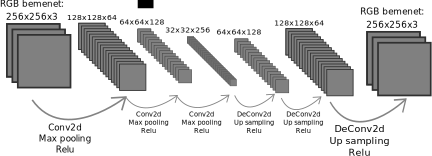
\includegraphics[scale=0.3]{img/autoencoder-network-modell.pdf}
	\caption{A háló modellje}
\end{figure}



%
%\lstset{language=Python}
%\begin{lstlisting}  
%
%	model = Sequential()
%	
%	kernel_sizes = [7, 7, 7]
%	kernel_dims = list(map(lambda x: (x,x), kernel_sizes))
%	iterator = iter(kernel_dims)
%	reverse_iterator = reversed(kernel_dims)
%	
%	padding = "same"
%	
%	padding_size = sum(kernel_sizes)*2
%	
%	model.add(ZeroPadding2D(padding=(padding_size, padding_size), input_shape=(None, None, 3)))
%	model.add(Conv2D(64, next(iterator), padding=padding))
%	model.add(Activation('relu'))
%	model.add(MaxPooling2D(pool_size=(2, 2)))
%	
%	model.add(Conv2D(128, next(iterator), padding=padding))
%	model.add(Activation('relu'))
%	model.add(MaxPooling2D(pool_size=(2, 2)))
%	
%	model.add(Conv2D(256, next(iterator), padding=padding))
%	model.add(Activation('relu'))
%	
%	# Visszaalakitas
%	
%	model.add(Conv2DTranspose(128, next(reverse_iterator), padding=padding))
%	model.add(Activation('relu'))
%	model.add(UpSampling2D(size=(2, 2)))
%	
%	model.add(Conv2DTranspose(64, next(reverse_iterator), padding=padding))
%	model.add(Activation('relu'))
%	model.add(UpSampling2D(size=(2, 2)))
%	
%	model.add(Conv2DTranspose(3, next(reverse_iterator), padding=padding))
%	model.add(Cropping2D(cropping=(padding_size, padding_size)))
%	
%	model.compile(
%		loss='mean_squared_error',
%		optimizer='adam', 
%		metrics=['accuracy']) 
%) 
%
%\end{lstlisting}


Az előző fejezet konvolúciós hálójához hasonlóan Konvolúció-Relu-MaxPooling hármasokat
fűztünk egymás után. Úgy találtuk hogy az általánosítás $ 7 \times 7 $-es kernelméret 
mellett volt optimális. Ha ennél kisebb volt, akkor túltanult, ha jelentősen nagyobb 
($ 11 $ és felette), akkor  már nem volt képes értékelhető eredményt adni.

A háló második fele az első fél tükrözve, figyelve arra, hogy a végső dimenzió pont akkora 
legyen, mint a bemenet. A \textit{Max poolingok} párja egy-egy \textit{Up sampling} réteg, amely az adott
pixelt egy $ 2 \times 2 $-es ablakban megtöbbszörözi.

Költségfüggvénynek átlagos hiba-négyzetet (\textit{MSE}) használunk, hiszen arra vagyunk 
kíváncsiak, hogy fizikailag mennyire voltunk közel az eredeti képhez.


Érdekessége a hálónak, hogy \textit{hely-invariáns}, azaz a kép koordinátáitól nem függ az adott
adategységhez tartozó kimenet, kizárólag a szomszédaitól és a megtanult szűrőktől.
Ezt ki is használjuk: az \texttt{ input\_shape=(None, None, 3)} utasítással annyit
specifikálunk csak, hogy az input 3 színcsatornával kell rendelkezzen, de tetszőleges
lehet a szélesség és a magasság. Ekkor bár az kötött, hogy tanításkor a példák egyforma 
dimenziójúak legyenek a hatékonyság miatt, de a méretük így is tetszőleges.


Megtehetjük tehát, hogy tanításnál sok kis kockát mutatunk a modellnek, viszont tesztelésnél
már az egész képet egyben használjuk, az eredmény ugyanaz lesz, mintha felkockáztuk 
és összeillesztettük volna. Ez magyarázható a konvolúció 
tulajdonságaival, erre alapul például jelfeldolgozásban az \textit{overlap-save} módszer.



\subsubsection{Osztályozás}

A háló kimenete az átlagos rekonstrukciós hiba. Az osztályozás ez alapján történik,
hasonlóan a \ref{sec:masodik.fazis} pontban leírtakhoz, azaz választunk egy küszöböt:
ha ez alatt van a hiba, akkor az eredetiség mellett döntünk, különben ellene.



\newpage
\section{Eredmények}

\subsection{SVM}
\label{sec:svm.eredmenyek}

Emlékezzünk vissza, hogy az SVM modellt azért kutattuk, mert egy kvázi kézzel írt elágazásokból 
álló, manuálisan felparaméterezett döntési folyamat elkészítését szerettük volna elsősorban
hatékonyabbá tenni, valamint automatizálni a modell újraillesztését adatokra, akkor is ha az 
adatbázis esetleg frissül, valamint hasonló új projekteknél ne kelljen elölről kezdeni a programozási
folyamatot, hanem legyen egy modulunk, amit csak fel kell paramétereznünk és be kell tanítanunk.


Az \ref{sec:svm.hiperparameter.optimalizalas} pontban leírtak miatt nem alkalmaztuk a szokásos 
\texttt{train-test-validation} hármast, mert statisztikai szempontból nem lett volna megbízható
az eredmény: túl sok múlott a szerencsén. Ez több adat beszerzésével működőképes módszer lesz,
addig is az átlagos hibarátát tekintettük mérvadó mérőszámnak.



\noindent
Az eredeti, gépi tanulás \textbf{nélküli} algoritmus eredményei, a minták \underline{darabszámában} 
kifejezve:

\begin{figure}[h!]
	\centering
	\begin{tabular}{ l l l l l }
		\underline{Adathalmaz}		& Összes minta 	& Bizonytalan	& Fals-pozitív	& Fals-negatív \\
		\texttt{bpas-verdict.csv}\footnotemark 	& 959 			& 206 			& 19	 	& 7			\\
		\texttt{bpas-merged.csv}\footnotemark[\value{footnote}] 	& 496			& 54 			& 16		& 1			\\
	\end{tabular}

	\caption{Az eredeti algoritmus eredményei}
\end{figure}

%\mbox{}
%
%\noindent
Ahogy a \ref{sec:dupla.kepes.eljaras} pontban írtuk, három módszer volt a tanításra.
Ezen algoritmusok eredményei hiba rátával kifejezve, és az eredetiekkel összehasonlítva:

\begin{figure}[h!]
	\centering
	\begin{tabular}{ l c c c c }
		\underline{Módszer} 		& Összes minta 	& Bizonytalan	& FP	& FN \\
		\texttt{bpas-verdict.csv}\footnotemark[\value{footnote}] 	& 959 			& 0.21			& 0.10215 	& 0.00905 	\\
		\texttt{bpas-merged.csv}\footnotemark[\value{footnote}] 	& 496			& 0.10			& 0.14545 	& 0.00259   \\
		
		\hline
		(1) verdict+SVM					& 894			& 0				& 0.00297	& 0.00566	\\
		(2) merged+SVM					& 453			& 0				& 0.01493	& 0.00771	\\
		(3) verdict+SVM 2 képpel		& 423			& 0				& 0.01420	& 0.01059   \\
		
	\end{tabular}

%	\begin{flushleft}
%	\textit{*Lásd a \ref{sec:adatok} pontot.}
%	\end{flushleft}
	\caption{Az SVM eredményei összehasonlítva az eredeti algoritmusokéval}

\end{figure}

\footnotetext{Lásd a \ref{sec:adatok} pontot.}
%\mbox{}



%\mbox{}



Láthatjuk, hogy az első modell érte el a legjobb eredményt, elsőfajú hibát tekintve minden mást megelőz, 
másodfajút mérve viszont nem tűnik jobbnak a \texttt{bpas-merged}-nél. Ez több mindennel magyarázható.
Láthatóan az algoritmus arra lett optimalizálva, hogy csökkenjen a másodfajú hiba, hiszen a 
\texttt{bpas-verdict}-hez képest nőtt az elsőfajú hiba rátája, pedig ez a több információt használó adat.
Emlékezzünk vissza, hogy nyomatoknál szívesebben engedünk át egy hamis példányt, mint utasítunk
el egy eredetit. Másodszor az adathalmaz fals-negatív elemszáma elég kicsi (1)- volt, ami 
statisztikailag nem elfogadható, ezért további vizsgálat szükséges ennek tényleges megállapítására.
Harmadszor az eredmény javítható lehet egy \textit{"bizonytalan"} halmaz bevezetésével, vagy 
a vágási pont eltolásával a másodfajú hiba javára.


Bár a második és a harmadik modell sem ért el rossz eredményt, de gyengébbek, mint az első. 
Az ott leírtak erre a két modellre is vonatkoznak. Az eredmények átlagolásánál szórást is mértünk, és azt tapasztaltuk, 
hogy az kétszerese az átlagnak, tehát relatív nagy. Ez azt jelentheti, hogy szerencsével és több 
újrafuttatással jobb modell is elérhető, de ez bizonytalan. Ha egy-egy tanítást nézünk, könnyen
találhatunk hibátlanul működő modellt. Ennek vizsgálata nagyobb és változatosabb adathalmazt igényel.

Általánosságban minden modellre elmondható, hogy több mintával pontosabb méréseket tudunk majd végezni.



%
% a dunno még csak benne sincs!
%
% eredményeket fenntartással kezelni, minél több mintha annál jobb lesz,
%de a kölönbözőség a fontos, nem a mennyiség
%
% ajnározni hogy ez mennyivel jobb mint az előző és tekintve hogy ez egy 
%próba projekt ígyéretes az eredmény
%
% meg kéne magyarázni mik azok a csv-k, valszeg még a megoldás részben
%ha uj feature kerül be arról is jó eséllyel jó lehet


%
%total samples:  419
%average+deviation type 1 error rate:
%0.0142 0.029636
%average+deviation type 2 error rate:
%0.01059 0.011837

\newpage
\subsection{Konvolúciós háló}
\label{sec:autoencoder.jelentoseg}
%2017_11_24__11_40_01.full_model.predictor.h5

A módszer sok szempontból kiválóan működött, de egy esetnél már a tanításnál elbukott. 
A tapasztalt jelenség az volt, hogy a háló, amelynek szerkezete nagyon hasonló volt 
a véglegeshez, egyáltalán nem akart tanulni: minden mintát hamisnak klasszifikált.
Eleinte azt hittük, hogy hibás a modell, ezért próbálkoztunk meg a \ref{sec:autoencoder}
fejezetben leírtak szerint egy autoencoderrel, amely a rekonstrukciós hibát méri.
Ennek eredményeit vizsgálva szembe tűnt, hogy a hamis minták egy halmaza egyáltalán nem 
tér el az eredetiektől. Ezek a hamis nyomatok az eredeti fájlokból lettek nyomtatva, 
tintasugaras nyomtatóval. Ezeket a Jurás algoritmus jó arányban meg tudta 
különböztetni az eredetiektől.


Az autoencoder bár önmagában is használható, de közel sem annyira megbízható, mint a többi 
módszer, így számszerű adatot nem is közlünk. A projekt szempontjából egy jelentős lépcső volt,
 ezért fontosnak tartottuk írni róla.

\label{sec:eredmenyek.100}
Amikor a fent említett hamis mintákat kivettük az tanító halmazból, a predikció elkezdett konvergálni,
ennek eredményeit láthatjuk a \ref{fig:roc-test}. és a \ref{fig:roc-full}. ábrán. A teszthalmaz szerencsésen
lett megválasztva, ami így 100\% os hatékonyságúnak bizonyult, ám mivel a tanító halmazon 
futtatva a modell mégsem tökéletes, fontosnak tartottuk azt is közölni. 



\begin{figure}[ht]
	

	\begin{minipage}[c]{0.5\linewidth}
		\includesvg[scale=0.5]{img/ruc-curve-test.svg}
%		\includegraphics[width=\linewidth]{img/ruc-curve-test.svg}
		\caption{Teszt halmaz}
		\label{fig:roc-test}

	\end{minipage}\hfill
	\begin{minipage}[c]{0.5\linewidth}
		\includesvg[scale=0.5]{img/roc-curve-full-dataset.svg}
%		\includegraphics[width=\linewidth]{img/ruc-curve-test.svg}
		\caption{Tanító+Teszt adathalmaz}
		\label{fig:roc-full}
		
	\end{minipage}
%	\caption{\textbf{Redukált feladat}}
%	\label{fig:redukalt.feladat}
\end{figure}


Ezután ebből a félkész a hálóból kiindulva megpróbáltuk továbbtanítani, újra a teljes adathalmazon,
amelyben a kritikus minták is szerepeltek. Jól látszott a véletlen szerepe a neurális 
hálók tanításában, ugyanis csak körülbelül tizedik próbálkozásra konvergált a modell a
jó irányba. Az első néhány próbálkozás a fentebb említett jelenséget produkálta: mindent 
hamisnak gondolt. Mindenesetre, végül sikerült a modellt ez alapján is betanítani, az 
eredmények pedig a \ref{fig:roc-test-re}. és a \ref{fig:roc-full-re}. ábrán láthatók.


Az eredményhalmaz szeparálhatóságát, és annak korlátait a \ref{fig:hist-test}. és a \ref{fig:hist-full}.
ábrán szemléltetjük, ahol egy hisztogramot láthatunk a \textit{Hamis} és az \textit{Eredeti}
halmazbeli értékek elhelyezkedéséről. Jól látható, hogy hol kell vágnunk, ha az 
első- vagy a másodfajú hibát szeretnénk csökkenteni. Ügyeljünk arra, hogy a hisztogram
logaritmikus skálát használ a jobb láthatóság kedvéért!


\begin{figure}[ht]
	
	
	\begin{minipage}[c]{0.5\linewidth}
		\includesvg[scale=0.5]{img/ruc-curve-test-ujratanitva.svg}
		%		\includegraphics[width=\linewidth]{img/ruc-curve-test.svg}
		\caption{Teszt halmaz}
		\label{fig:roc-test-re}
		
	\end{minipage}\hfill
	\begin{minipage}[c]{0.5\linewidth}
		\includesvg[scale=0.5]{img/roc-curve-full-dataset-ujratanitva.svg}
		%		\includegraphics[width=\linewidth]{img/ruc-curve-test.svg}
		\caption{Tanító+Teszt adathalmaz}
		\label{fig:roc-full-re}
		
	\end{minipage}
%	\caption{\textbf{Újratanított háló}}
	\label{fig:ujratanitott.feladat}
\end{figure}



\begin{figure}[ht]
	
	
	\begin{minipage}[c]{0.5\linewidth}
		\includesvg[scale=0.5]{img/histogram-ujratanitott-log-skala-test.svg}
		%		\includegraphics[width=\linewidth]{img/ruc-curve-test.svg}
		\caption{Teszt halmaz}\label{fig:hist-test}
		
	\end{minipage}\hfill
	\begin{minipage}[c]{0.5\linewidth}
		\includesvg[scale=0.5]{img/histogram-ujratanitott-log-skala-full.svg}
		%		\includegraphics[width=\linewidth]{img/ruc-curve-test.svg}
		\caption{Tanító+Teszt adathalmaz}\label{fig:hist-full}
		
	\end{minipage}
%	\caption{\textbf{Az újratanított háló predikciós hisztogramja}}
	\label{fig:histogram-ujratanitott}
\end{figure}


Végül nézzük az összehasonlítást az eredeti, gépi tanulást nélkülöző algoritmusokkal:

\begin{figure} [h!]
	\centering
	\begin{tabular}{ l c c c c  }
		\underline{Módszer} 			& Összes minta 	& Bizonytalan	& FP	& FN \\
		\texttt{bpas-verdict.csv}\footnotemark 	& 959 			& 0.21			& 0.10215 	& 0.00905 	\\
		\texttt{bpas-merged.csv}\footnotemark[\value{footnote}]  	& 496			& 0.10			& 0.14545 	& 0.00259   \\
		
		\hline
		Konvolúviós háló redukálva\footnotemark 	& 894			& 0				& 0.02798	& 0.00972	\\
		Konvolúviós háló újratanítva& 894			& 0				& 0.05555	& 0.00900	\\
		
		
	\end{tabular} 

	\caption{A mély konvolúciós háló eredményei}
%	\caption{A mély konvolúciós háló eredményei összehasonlítva az eredeti algoritmusokéval}
\end{figure}

\addtocounter{footnote}{-1}
\footnotetext{Lásd a \ref{sec:adatok} pontot.}
\addtocounter{footnote}{1}
\footnotetext{A fentiek szerint szűrt mintákon.}


%\textit{*Lásd a \ref{sec:adatok} pontot.}
%
%\textit{**A fentiek szerint szűrt mintákon.}


Összességében azt mondhatjuk, hogy a konvolúciós háló jól teljesített, megállja a helyét 
a többi algoritmus között, az átlagos hamisítványokat nem engedi át, eredetit csak ritkán 
osztályoz félre. Ne felejtsük el, hogy több tanító példával jobb eredmény várható,
valamint elképzelhető, hogy a hiperparaméterek további optimalizálásával és a háló 
szerkezetének alakításával megbízhatóbb osztályozó képességet lehet elérni. 
Továbbá ez a megoldás nem használja ki, hogy két képet készítünk, tehát ezzel még 
tudunk javítani a teljesítményen. További munkát igényel, hogy kidolgozzunk valamilyen
módszert arra, hogy konvolúciós hálókkal a fent említett kritikus hamisítványokat megfogjuk.
Nem elképzelhetetlen, hogy az eredeti algoritmusokkal, vagy azok SVM-el módosított változataival
párhuzamosan használjuk.




%(0.027985074626865673, 0.0097205346294045869, 0.50870099999999996)
%0.055555555555555552, 0.009009009009009028
%
%100\% lett a teszt halmazon - 120 mintából
%
%az autoencoder segített ráönni, hogy hol lett elbaszva
%nem használtuk ki hogy két képünk van
%
%
%további kutatás: további mintákkal-
%az eredményt a helyén kell kezelni - de azért bíztató
%limitáció - az offsetet nem fogta meg
%
%
%2 image merge vs sima - mi is 2 képet használtunk
%összehasonlítani a jurás eredménnyel
%
%megnézni mennyire függ a mázlitól a tanítás
%validációs hiba vs rendes hiba
%
%párhuzamosan használni a kézi elemzéssel










\newpage
\section{Konklúzió}


Bátran állíthatjuk, hogy a Gépi Tanulásnak van helye az eredetiség vizsgálat témakörében.
Igaz, a módszer még nem elég kifinomult ahhoz, hogy azonnal ipari környezetben használjuk,
de azt mindenképpen bizonyítottunk, hogy ígéretes kutatási terület, és lehet jövője éles 
helyzetekben is.


Az SVM, vagy akár egyéb gépi tanulásra alapuló algoritmus tökéletesen illeszkedik
a döntéshozás munkamenetébe, és kétség sem fér a hasznosságához. A kockázata sem 
túl nagy, hiszen a működési mechanizmusa hasonlít ahhoz, amit egy programozó kézzel írna.
Az SVM jó tulajdonsága a magyarázó képesség. Egy neuronhálóval ellentétben, ha rátekintünk
a paramétereire meg tudjuk mondani, hogy egy adott döntést miért hozott, és ha ezzel nem vagyunk 
elégedettek tudjuk, hol kell javítani.


Egy konvolúciós háló sokkal erőforrás-igényesebb, és egy teljesen más megközelítés,
amely még csak nem is hasonlít az eddig használt algoritmusokhoz, ezért óvatosan kell 
kezelni. Hátránya, hogy nehéz kinyomozni, hogy mi az oka annak, ha valami nem működik,
azaz ahogy fentebb említettük
kifejezetten rossz a magyarázóképessége. Problémát okozhat a használata kis erőforrással 
rendelkező rendszerekben: GPU nélkül nem érdemes használni. A rejtett rétegek súlyai is 
meglehetősen sok helyet foglalnak: jelen pillanatban 120 megabájt körül van, de ha tegyük
fel egy telefon makrolencsével készült teljes képét ki szeretnénk elemezni, 
amelyek csúcskategóriás készülékeknél bőven 10 megapixel felett van, akkor hatalmasra 
nőhet a belső reprezentáció. Véleményem szerint még több évnyi munka kell ahhoz, hogy 
ebből egy megbízható alkalmazás legyen, ami minden körülmények között meg tud 
különböztetni egy hamis nyomatot egy eredetitől.


\subsection{További feladatok}

Amennyiben ebből használható alkalmazást szeretnénk készíteni át kell ültetnünk mobil 
platformra. Nem kétséges, hogy a mai mobil GPU-k már hatékonyan fognak megbirkózni a
feladattal. Ne felejtsük el, hogy bár egy neuronhálót betanítani idő- és erőforrás-igényes,
használni már jóval egyszerűbb, feltéve, hogy a modellt egy az egyben beleépítjük a használó
alkalmazásba.


A dolgozathoz a projekt \texttt{pythonban} készült. Ez egy rendkívül flexibilis nyelv, és
kiváló prototípus készítéshez, de tekintve, hogy egy szkriptnyelv, a hibakezelés a 
típusosság hiányában sokkal nehezebb. Emiatt célszerűnek látom az éles környezetben 
való használathoz egy fordítóval rendelkező, biztonságos, de mégis hatékony nyelven 
való megvalósítását, erre \texttt{C++}-t javaslok. Ehhez létezik kiegészítő könyvtár,
amivel a \texttt{Keras} által készített modellt használni tudjuk, valamint az 
ehhez szükséges 
\texttt{Tensorflow} csomag szintén elérhető.


Preferenciáktól függő feladat egy \textit{Bizonytalan} intervallum bevezetése minden
projekthez, amelyhez szükségünk van egy maximálisan eltűrt első- és másodfajú hibarátára.

\subsection{Kutatási területek}

A képek normalizálása során felmerült, hogy bár a pozicionáló koordináták rendelkezésünkre 
álltak, a konvolúciós hálók alkalmasak lehetne ezek hatékony megtalálására.


Ahogy az eredményeknél elemeztük, kutatást igényel bizonyos képek elemzése,
ez még a jövő feladata.

%
%további feladatok:
%
%például mobilra átültetni
%dunno bevezetése
%emberi programozási nyelv - ez csak prototípus annak minden bajával
%
%
%lehetne majd pozicionálásra is megpróbálni
%
%
%kis kikockázás
%
%batch, eposz
%dropout, normalizálás, balancing, augmentation
%loss/accuracy - roc görbe "siker mérése"
%test/val/train
%early stopping
%MERGED images??? dunno?


\newpage
\section{Fejlesztői dokumentáció}

A forráskódok a \url{https://github.com/csatacsirke/diplomamunka/} weboldalon érhetőek el.


\textit{Megjegyzés}: Tekintve, hogy a projekt nem egy végfelhasználói alkalmazás, hanem 
egy prototípus, a kódhoz nem mellékelünk felhasználói dokumentációt.


A projektet \texttt{python} nyelven készítettük. Ez kiválóan alkalmas prototípusok készítésére, amelyeket újrafordítás nélkül, akár egy-egy sort futtatva azonnal kipróbálhatunk. A  háttérkönyvtáraknak köszönhetően, amelyek natív kóddá fordítják a kritikus, számításigényes részeket, a  teljesítmény sem romlik jelentősen. Ezek alapján nem meglepő, hogy a legtöbb gépi tanulással foglalkozó programcsomagnak létezik \texttt{python} interfésze.


Mi \texttt{WinPython 3.5.4}\footnote{\url{https://winpython.github.io/}} disztribúciót használtunk, de bármelyik másik \texttt{python 3.x} jó lett volna. A szerző személyes tapasztalatai miatt Visual Studio IDE-ben fejlesztettünk. Emiatt a projekt könyvtárában található egy \texttt{.sln} és egy \texttt{.pyproj} fájlt, amelyek tartalmazzák a szükséges konfigurációkat a fejlesztőkörnyezet számára. Ezeket használva a program alapértelmezés szerint a \texttt{./working\_dir/} könyvtárban fut, valamint ott keres minden szükséges bemenetet, és ez a relatív elérési útvonalak alapja.


A szkriptek platformfüggetlenek, futtatásukhoz a \texttt{pythonon} és annak megfelelő csomagjain 
kívül nem szükséges egyéb keretrendszer, azok parancssorból futtatva is működnek.


\subsection{Felhasznált csomagok}

\texttt{Python} csomagokat a \texttt{pip}\footnote{\url{https://pypi.python.org/pypi/pip}} segítségével tudunk telepíteni, mely a 
disztribúciónkban \texttt{/Scripts/pip.exe} néven található meg. Ehhez a következő parancsot
használjuk:

\begin{lstlisting}  
	>pip install <csomag neve>
\end{lstlisting}

Ekkor a rendszer letölti a csomagot annak minden függőségével együtt, gondoskodva a megfelelő
verziókról is. 

\subsubsection{NumPy}

Általános matematikai csomag, széles körű függvénykínálattal.
Szinte minden más, általunk használt csomag erre épül.


\subsubsection{SciPy}

Tudományos csomag, általános funkciókkal. Sok más magasabb szintű csomag épül rá. Mi például
a \texttt{matplotlib} könyvtárát használtuk diagramjaink készítéséhez.


\subsubsection{TensorFlow}

Elosztott matematika könyvtár, amely lehetővé teszik bonyolult számítások párhuzamosított
elvégzését heterogén platformokon. Mi ezt csak közvetve használjuk a magasabb szintű 
könyvtárak által, kivéve mikor a maximális memóriaméretet állítjuk be, ahogyan arról a 
\ref{gpu.memory}. fejezetben írtuk. Létezik külön CPU és GPU változata, erről később a 
\ref{sec:gpu.kovetelmenyek}. pontban írunk részletesebben.



\subsubsection{Sklearn} 

Egy nyílt forráskódú, \texttt{python} alapú gépi tanulási algoritmusokat nyújtó csomag. 
Az SVM osztályozáshoz ezt használtuk.


\subsubsection{Keras}

Magas szintű könyvtár neuronhálók építéséhez. Válaszható, hogy milyen alacsony szintű
aritmetikai könyvtárat használjon, mi a fent említett \texttt{TensorFlow}-t választottuk.
A konvolúciós hálónkat ezzel készítettük.

\subsubsection{OpenCV}

Számítógépes látáshoz írt képkezelő könyvtár. Lényegében minden meg van benne, ami egy
átlagos képszerkesztő programban. Ennek segítségével töltjük be a képeket, valamint 
ezzel számoljuk ki és végezzük el a normalizáláshoz szükséges perspektív transzformációt.


\subsubsection{Hyperopt}

\subsection{Futtatás a videókártyán}
\label{sec:gpu.kovetelmenyek}

Ahogy a fejezet elején írtuk, a projekt használatához csak \texttt{pythonra} van szükség,
de ez csak akkor igaz, ha megelégszünk azzal, hogy a program a CPU-n fut. A GPU 
használatba vételéhez további komponensek szükségesek.


Először is szükségünk van egy \texttt{CUDA}-t támogató videókártyára, erre viszont jelenleg csak
az Nvidia kártyák képesek. Ezután fel kell telepítenünk a CUDA fejlesztő csomagját (SDK), ami a
GPU általános célú programozását teszi lehetővé. 


Ekkor már feltelepíthetjük a \texttt{Tensorflow} GPU-s változatát:
\begin{lstlisting}
	>pip3 install --upgrade tensorflow-gpu
\end{lstlisting}



Ezután fel kell telepítenünk a cuDNN könyvtárat (CUDA Deep Neural Network library), 
mely hatékony neurális hálóval kapcsolatos algoritmusokat válósít meg. Ezeket a 
\texttt{Keras} használja.


Előfordulhat, hogy az \texttt{Nvidia} szoftverek telepítésekor nem adódnak hozzá a 
Windows \texttt{PATH} környezeti változójához. Ekkor ezt nekünk kézzel kell megtennünk,
különben a \texttt{python} nem fogja ezeket megtalálni.


\subsection{Szerkezet}

A projekt \texttt{python} forrásfájlokból áll. Ebből az alábbi négy futtatható:


\begin{itemize}
	\item \texttt{cnn.py}
	\item \texttt{statistics.py}
	\item \texttt{verdict\_nn.py}
	\item \texttt{batch\_normalize.py}

\end{itemize}

A többi fájl csak segédfüggvényeket tartalmaz.

\subsection{cnn.py}

Ez a konvolúciós háló belépési pontja, ezzel tudunk tanítani és kiértékelni. Tekintve, hogy 
a programunk nem egy végfelhasználói alkalmazás, és hogy egy szkriptnyelvvel dolgozunk nincs 
felhasználói felület. A szkript első néhány sorában, a függőségek után találjuk a bemeneti 
paramétereket. Ezek közül a következők fontosak:
%Ezek közül a fontosak a következők:

\subsubsubsection{use\_autoencoder : bool}

Meghatározza, hogy a modell autoencoder vagy predikciós legyen.



\subsubsubsection{recalculate : bool}

Ha ez be van kapcsolva, akkor a program új modellt épít akkor is, ha talált volna 
már meglévőt amit betölthet és használhat.


\subsubsubsection{stage : int $ \in \{1, 2\} $}

A program két fázisból áll, egy tanításiból és egy kiértékelésiből. Ha ez a paraméter
$ 2 $, akkor átugorjuk a tanítási fázist. Ekkor a \texttt{recalculate} paraméternek
hamisnak kell lennie, és léteznie kell egy korábban elmentett modellnek, amit be
tudunk tölteni.



\subsubsubsection{weights\_only : bool}

Ha ez be van kapcsolva, akkor mentéskor csak a modell súlyai maradnak meg. Ellenkező esetben
a modell struktúrája, a tanítás teljes munkamenete, valamint az optimalizáló állapota is.
Csak akkor érdemes használni, ha egy végleges alkalmazást készítünk, aminek tárhely-hatékonynak 
kell lennie.


\subsubsubsection{weight\_file : String?}

%A program, amikor egy előző modellt próbál betölteni megkeresi a dátum szerint utolsó
Amikor a program egy előző modellt próbál betölteni, megkeresi a dátum szerinti utolsó
fájlt, és azzal próbál dolgozni. Lehetőségünk van ezt felülbírálni, és a modell elérési
útvonalát explicit megadni. Ha nem szeretnénk használni, állítsuk az értékét \texttt{None}-ra.


\subsubsubsection{default\_input\_file\_name: String}

Egy olyan \texttt{.csv} fájlra kell mutatnia, amelynek első oszlopa képek elérési útvonala,
a második pedig egy azonosító arról, hogy az adott kép eredeti~(0) vagy hamis~(1) nyomatról készült.
Ezt csak az első futtatáskor használjuk, amikor a tanító-, validációs- és teszthalmazokat 
generáljuk. Amint ezek elkészültek elmentjük őket egy külön fájlba, amit minden futtatás elején
betöltünk. Ezt a \texttt{dataset\_handler.py} modul \texttt{load\_dataset\_or\_create\_new} 
automatikusan elvégzi nekünk.


\subsubsubsection{use\_full\_dataset\_for\_test : bool}

Ha igazra van állítva, akkor nem csak a teszthalmazra futtatja le a kiértékelést, hanem 
a teljes adatmennyiségre. 


\subsubsection{Működés}

Ha a fenti paramétereket beállítottuk, akkor rendelkezésünkre állnak a képek elérési
útvonalai, és a hozzájuk tartozó igazságértékek. Ezután betöltjük vagy elkészítjük a 
modellünket. A fenti paraméterek alapján kiválasztjuk milyen sémát használunk: 
\texttt{Autoencoder}-t vagy \texttt{Predictor}-t. Ez a \texttt{Scheme} osztály végzi a háló
modelljének építését. Ha a modell elkészült, akkor készen állunk a munkára.


%Ha az első fázisban vagyunk, akkor a \texttt{model.fit\_generator} függvényét hívjuk meg
Az első fázisban a \texttt{model.fit\_generator} függvényét hívjuk meg
%a tanítás elkezdéséhez. A tanulás és a megállás a \ref{sec:cnn}. fejezetben ismertetettek 
a tanítás elkezdéséhez, amely a \ref{sec:cnn}. fejezetben ismertetettek szerint történik.


A második fázisban a modellt a \texttt{Scheme.eval} függvény értékeli ki. A teszthalmaz 
minden elemére elvégzi az osztályozást, majd az eredményt egy \texttt{.csv} fájlba írja, így ezután a statisztikai vizsgálat a háló használata nélkül is elvégezhető.
%Ezután ez a háló további használata nélkül is vizsgálható statisztikai szempontok alapján.



\subsection{statistics.py}

A \texttt{cnn.py} szkript kimenetét elemezi és vizualizálja. 
A parancssori bemenete egy \texttt{.csv} fájl, amelyet elemezni fog. Amennyiben ez hiányzik, úgy az időben utolsó, \texttt{.stage2.csv}-re végződő fájlt tölti be a futtatási könyvtárból.
%A bemenete egy \texttt{.csv} 
%fájl, amit vagy parancssori paraméterként kap, vagy amennyiben ez hiányzik, az időben utolsó,
%\texttt{.stage2.csv}-re végződő fájl a futtatási könyvtárban.


Futtatás során bemenethez kiszámolja a hozzá tartozó ROC-görbét, legkisebb hibarátát,
és ehhez megadja az első- és másodfajú hibarátát. Ezen felül hisztogramot készít a 
két osztály eloszlásáról, majd mindezeket diagramokon megjeleníti. Ezt a modult használtuk
a dolgozatban szereplő ábrák elkészítéséhez.


\subsection{verdict\_nn.py}

Az SVM tanításáért és kiértékeléséért felelős modul. A konvolúciós hálóval ellentétben
ez nem lett ketté bontva. Ennek első oka, hogy sokkal gyorsabb a tanítás: a tesztgépen 
a másodperc törtrésze. Másodszor, a statisztikák készítésekor tömegesen újratanítottuk a 
modellt különböző adatokon, hogy mérjük a véletlen szerepét. Erről részletesen 
az \ref{sec:svm.eredmenyek}. fejezetben olvashatunk.

\subsubsection{Paraméterek}

A konvolúciós hálóhoz hasonlóan néhány paraméter a szkript elején található. Ezek közül
lássuk a lényegeseket:

\subsubsubsection{mode : int $ \in \{1, 2, 3\} $}

Értékétől függ mit fogunk számolni.
\begin{enumerate}
\item 
	\texttt{mode\_fit\_and\_test}: Az input alapján betanít egy SVM-et és értékeli azt.
\item
	 \texttt{mode\_batch\_fit\_and\_test}: Az input alapján több SVM-et tanít és az eredményeiket átlagolja.
	 Ennek szükségességét az eredmények fejezetben tárgyaltuk.
\item 
	\texttt{mode\_hyperopt}: Az input alapján megkeresi a legjobb hiperparamétereket. 
	Erről részletesen a \ref{sec:svm.hiperparameter.optimalizalas}. fejezetben írtunk.
\end{enumerate}


\subsubsubsection{use\_two\_images : bool}

%Ha ez a paraméter be van kapcsolva, akkor megkíséreljük a szomszédos képek összefűzését, ahogy azt
Ha ez \texttt{True}, akkor megkíséreljük a szomszédos képek összefűzését, ahogy azt
a \ref{sec:dupla.kepes.eljaras}. pontban részleteztük.


\subsection{batch\_normalize.py}

Ahogy azt korábban írtuk, a képeket a célzókörök alapján normalizáltuk, de ez rendkívül 
erőforrás-igényes lett volna futási időben, ezért ezt már tanítás előtt lefuttattuk minden
mintára. Ennek megvalósítására szolgál ez a szkript. A bemenetként kapott \texttt{.csv} 
fájl által hivatkozott minden képhez elkészíti annak normalizált változatát, majd elmenti
az eredetiek mellé, egy \texttt{"normalized\_"} előtaggal.

Amennyiben a célzókörök koordinátái nem álltak rendelkezésre egy-egy képhez, úgy azok nem
lettek figyelembe véve.


\subsection{Egyéb forrásfájlok}

A következő szkriptek önmagukban nem futtathatóak, csak segédfüggvényeket tartalmaznak.

\begin{itemize}
\item 
	\texttt{dataset\_handler.py}: A tanító-, validációs- és teszthalmazok kezeléséért felelős.
\item 
	\texttt{image\_processing.py}: Képmanipuláló algoritmusok.
	
\item 
	\texttt{log.py}: Azért felelős, hogy a program üzenetei mind a képernyőn, mind 
	az aktuális logfájlban megjelenjenek.
\item 
	\texttt{util.py}: Általános használatú, más modulba nem illő függvényeket tartalmaz.
\end{itemize}


%
%\subsection{TODO}
%
%akár az argparse is mehet
%numpy
%keras
%sklearn
%tensorflow
%cuda
%cuda nn
%winpython 3.6
%hyperopt
%matplotlib
%opencv
%visual studio - working dir
%csomagokhoz->pip

\newpage
%\begin{thebibliography}{99}
%	\bibitem{adam} 
%	Diederik P. Kingma, Jimmy Ba:
%	Adam: A Method for Stochastic Optimization
%	arXiv:1412.6980v9 [cs.LG]
%	
%	
%	\bibitem{okostelefonnal.a.csomagolas.vedelmeert} 
%	Okostelefonnal a csomagolás védelméért
%	Szerző: Gyenes András
%	Megjelent: MAGYAR GRAFIKA 2016/2	
%%	
%%	@article{yeh2011employing,
%%		title={Employing multiple-kernel support vector machines for counterfeit banknote recognition},
%%		author={Yeh, Chi-Yuan and Su, Wen-Pin and Lee, Shie-Jue},
%%		journal={Applied Soft Computing},
%%		volume={11},
%%		number={1},
%%		pages={1439--1447},
%%		year={2011},
%%		publisher={Elsevier}
%%	}
%
%	
%\end{thebibliography}

\bibliographystyle{plain}
\bibliography{tex/references}{}




% TODO github linket belerakni


%I think we did a pretty good\textsuperscript{\textit{job}}so far

